\documentclass[11pt]{jarticle}

\usepackage[dvipdfmx]{graphicx}

\setlength{\oddsidemargin}{-6.35mm}
\setlength{\textwidth}{171.9mm}

\begin{document}

\title{画像処理実験 最終レポート}
\author{09430509\\今田将也}
\date{\number\year 年\number\month 月\number\day 日}
\maketitle

本実験では,複数の画像を合成して広い範囲の映ったパノラマ画像を作成し,より正確な合成を行う方法を学ぶ.
各時間ごとの課題の考察について述べたあと,最終的なパノラマ画像の合成結果について述べる.

\section{画像フォーマット / 画像の表示}
計算機で画像を扱うには,次のようなことを理解する必要がある.プログラム内部で画像を表現する際のデータ構造.画像ファイル入出力の方法と画像圧縮.画像処理の方法.

\subsection{課題 配列の数値を書き換え,適当に編集して,画像をレポートに挿入しなさい.}
画素が白か黒等の2種類の画像を2値画像と呼ぶ.
画像の大きさのうち、横の画素数を幅(width),縦の画素数を高さ(height)と呼ぶ.
各画素の色は1つの数値で表される.これらの数値を画素値あるいは輝度値(intensity value)等と呼ぶ.通常,画素値は8ビット符号なし整数(unsigned char)である.画素値の最小値が黒,最大値が白,中間の値が様々な濃さの灰色を表すような画像を濃淡画像と呼ぶ.

カラー画像の各画素は光の三原色(赤R, 緑G, 青B)の各成分からなり,画素が極めて小さいとき加法混色によって様々な色に見える.カラー画像の配列表現法は複数の種類がある.一つは,各画素に対して R, G, B の輝度を並べる方法である.

画像の編集をした結果を図\ref{1-1.png},図\ref{1-2.png},図\ref{1-3.png}に示した.

\begin{figure}[htbp]
    \begin{tabular}{ccc}
        \begin{minipage}{0.33\hsize}
            \begin{center}
                
\includegraphics[scale=.5]{1-1.png}
                \caption{1-1の画像}
                \label{1-1.png}
            \end{center}
        \end{minipage}
        \begin{minipage}{0.33\hsize}
            \begin{center}
                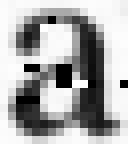
\includegraphics[scale=.5]{1-2.png}
                \caption{1-2の画像}
                \label{1-2.png}
            \end{center}
        \end{minipage}
        \begin{minipage}{0.33\hsize}
            \begin{center}
                
\includegraphics[scale=.5]{1-3.png}
                \caption{1-3の画像}
                \label{1-3.png}
            \end{center}
        \end{minipage}
    \end{tabular}
\end{figure}

\subsection{カラー画像から R, G, B への分解}
以下のように,配列dstのp+0要素の赤成分のみを代入することで実装した.
また,p+1要素,p+2要素にsrc[p+0]を代入することで緑成分のみ,青成分のみを取り出した.

\begin{verbatim}
    (プログラム一部省略)
    dst[p+0]=src[p+0];
    dst[p+1]=0;
    dst[p+2]=0;
\end{verbatim}
\begin{figure}[htbp]
    \begin{tabular}{ccc}
        \begin{minipage}{0.33\hsize}
            \begin{center}
                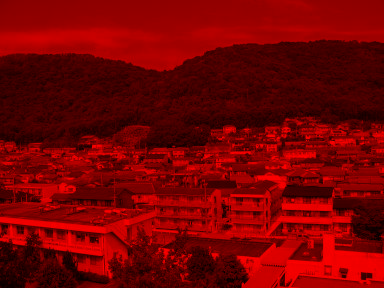
\includegraphics[scale=.3]{1-4.png}
                \caption{赤色の画像}
            \end{center}
        \end{minipage}
        \begin{minipage}{0.33\hsize}
            \begin{center}
                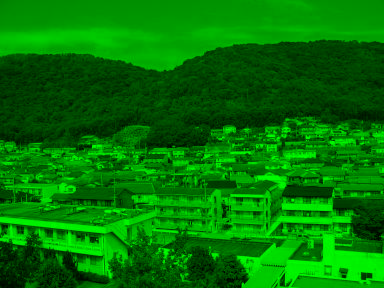
\includegraphics[scale=.3]{1-4-1.png}
                \caption{緑色の画像}
            \end{center}
        \end{minipage}
        \begin{minipage}{0.33\hsize}
            \begin{center}
                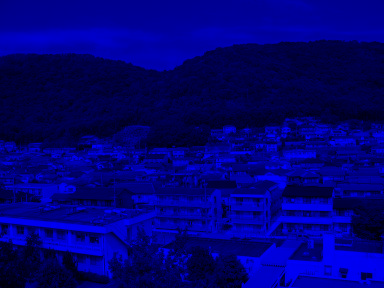
\includegraphics[scale=.3]{1-4-2.png}
                \caption{青色の画像}
            \end{center}
        \end{minipage}
    \end{tabular}
\end{figure}

\subsection{画像の拡大}
画像の拡大をするために,画像の色を抽出する手順の前に拡大を行う手順を入れた.
以下はそのソースコードを一部抜粋した.

\begin{verbatim}
    //拡大
    var xx=Math.round(x/4)+200,yy=Math.round(y/4)+100;
    q=(wdt*yy+xx)*4;
    dst[p+0]=src[q+0];
    dst[p+1]=src[q+1];
    dst[p+2]=src[q+2];

    //色の抽出
    p=(y*wdt+x)*4;
    dst[p+0]=r/49;
    dst[p+1]=g/49;
    dst[p+2]=b/49;
    dst[p+3]=255;
\end{verbatim}
\begin{figure}[h]
    \centering
    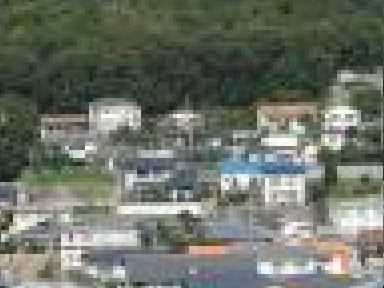
\includegraphics[scale=.3]{1-4-3.png}
    \caption{4倍に拡大した画像}
\end{figure}

\subsection{C言語で画像処理}
講義のページにあるimage.h,image.c,image2.c,image2.cxxを利用し,
easyProcess.cを作成後以下のコマンドにて実行をおこなった.

\begin{verbatim}
    $ gcc --no-warnings -O easyProcess.c image.c image2.c
    $ ./a.out 0.jpg a.jpg
\end{verbatim}

生成された画像を図\ref{1-5.jpg}に示した.
\begin{figure}[htbp]
    \centering
    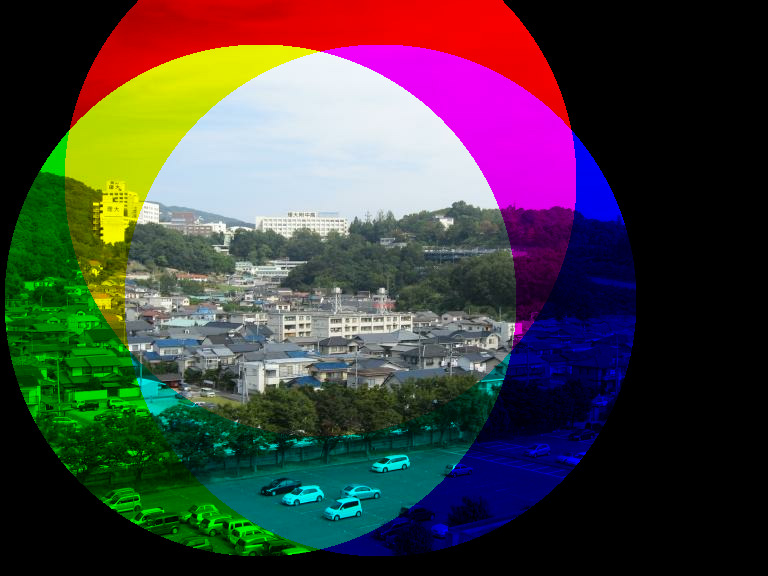
\includegraphics[scale=.2]{1-5.jpg}
    \caption{easyProcessにて生成された画像}
    \label{1-5.jpg}
\end{figure}

\subsubsection{赤色のみ抽出}
IElem(dst,x,y,0)にIElem(src,x,y,0)で赤要素のみを入れた.緑と青に関しては,
例のように0を入れるつまり無視すれば良いので,コメントアウトすることで実装した.
図\ref{1-6.jpg}に示す

\begin{figure}[htbp]
    \centering
    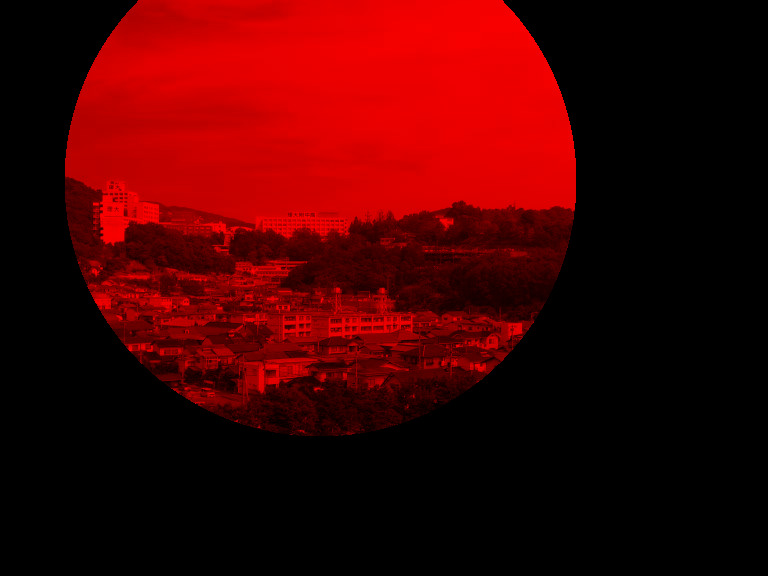
\includegraphics[scale=.2]{1-6.jpg}
    \caption{赤色のみ抽出した画像}
    \label{1-6.jpg}
\end{figure}

\subsubsection{緑色のみ抽出}
赤色のときと同様の方法で実装した.
図\ref{1-7.jpg}に示す

\begin{figure}[htbp]
    \centering
    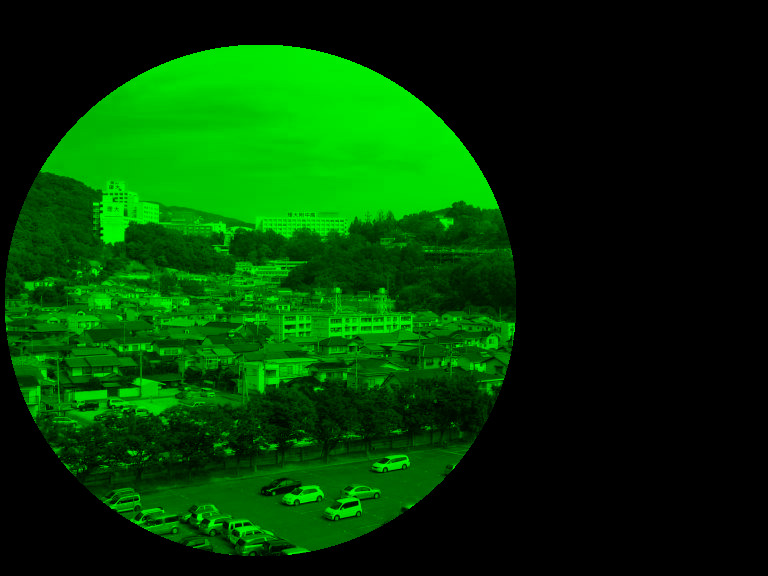
\includegraphics[scale=.2]{1-7.jpg}
    \caption{緑色のみ抽出した画像}
    \label{1-7.jpg}
\end{figure}

\subsubsection{青色のみ抽出}
赤色のときと同様の方法で実装した.
図\ref{1-8.jpg}に示す

\begin{figure}[htbp]
    \centering
    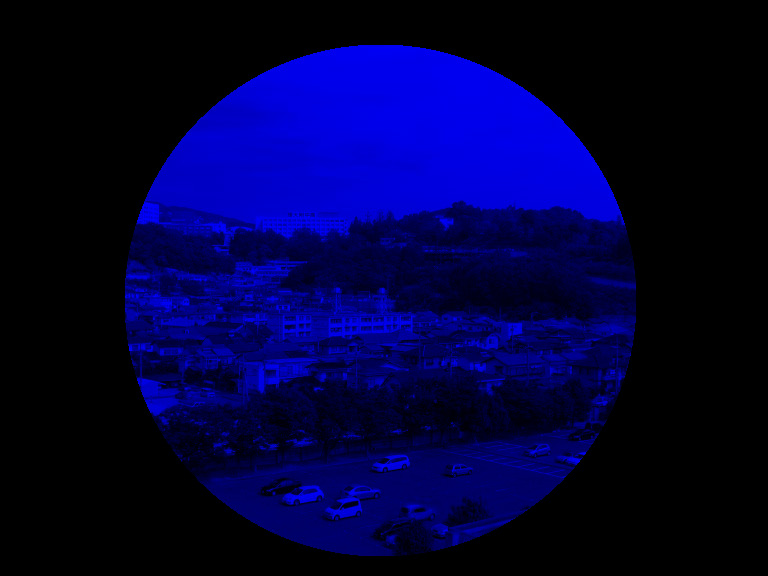
\includegraphics[scale=.2]{1-8.jpg}
    \caption{青色のみ抽出した画像}
    \label{1-8.jpg}
\end{figure}

\subsubsection{画像の拡大}
画像の拡大は,IElemのsrcで指定されている箇所のxとyをそれぞれ変更することで
拡大の実装ができる.以下そのコードを一部抜粋したものである
\begin{verbatim}
    int qx = round((x)/2);
    int qy = round((y)/2); 
    IElem(dst,x,y,0) = IElem(src,qx,qy,0)*disk(x,y,320,180)/256; // red at (x,y)
\end{verbatim}
また,その結果の画像を図\ref{1-9.jpg}に示す.
\begin{figure}[htbp]
    \centering
    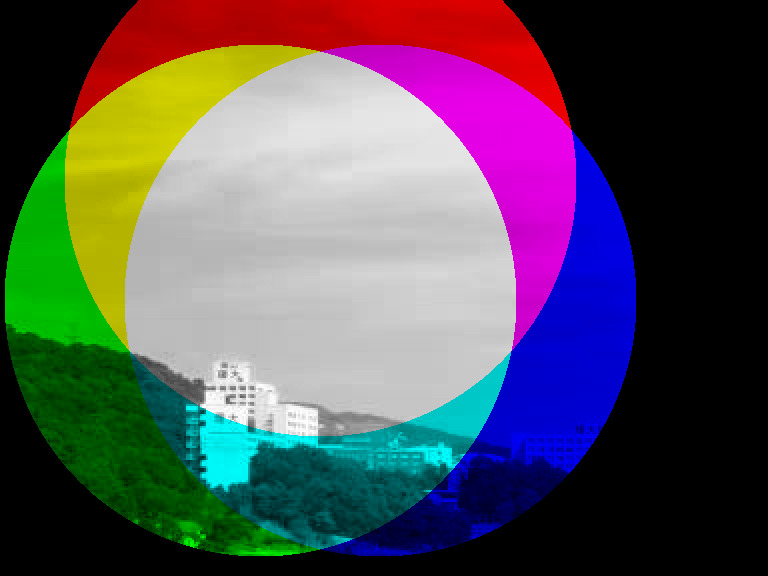
\includegraphics[scale=.2]{1-9.jpg}
    \caption{拡大した画像}
    \label{1-9.jpg}
\end{figure}

\subsubsection{スマホで撮影した画像での実験}
実験元の画像を図\ref{1-10.jpg}に示す.
\begin{figure}[htbp]
    \centering
    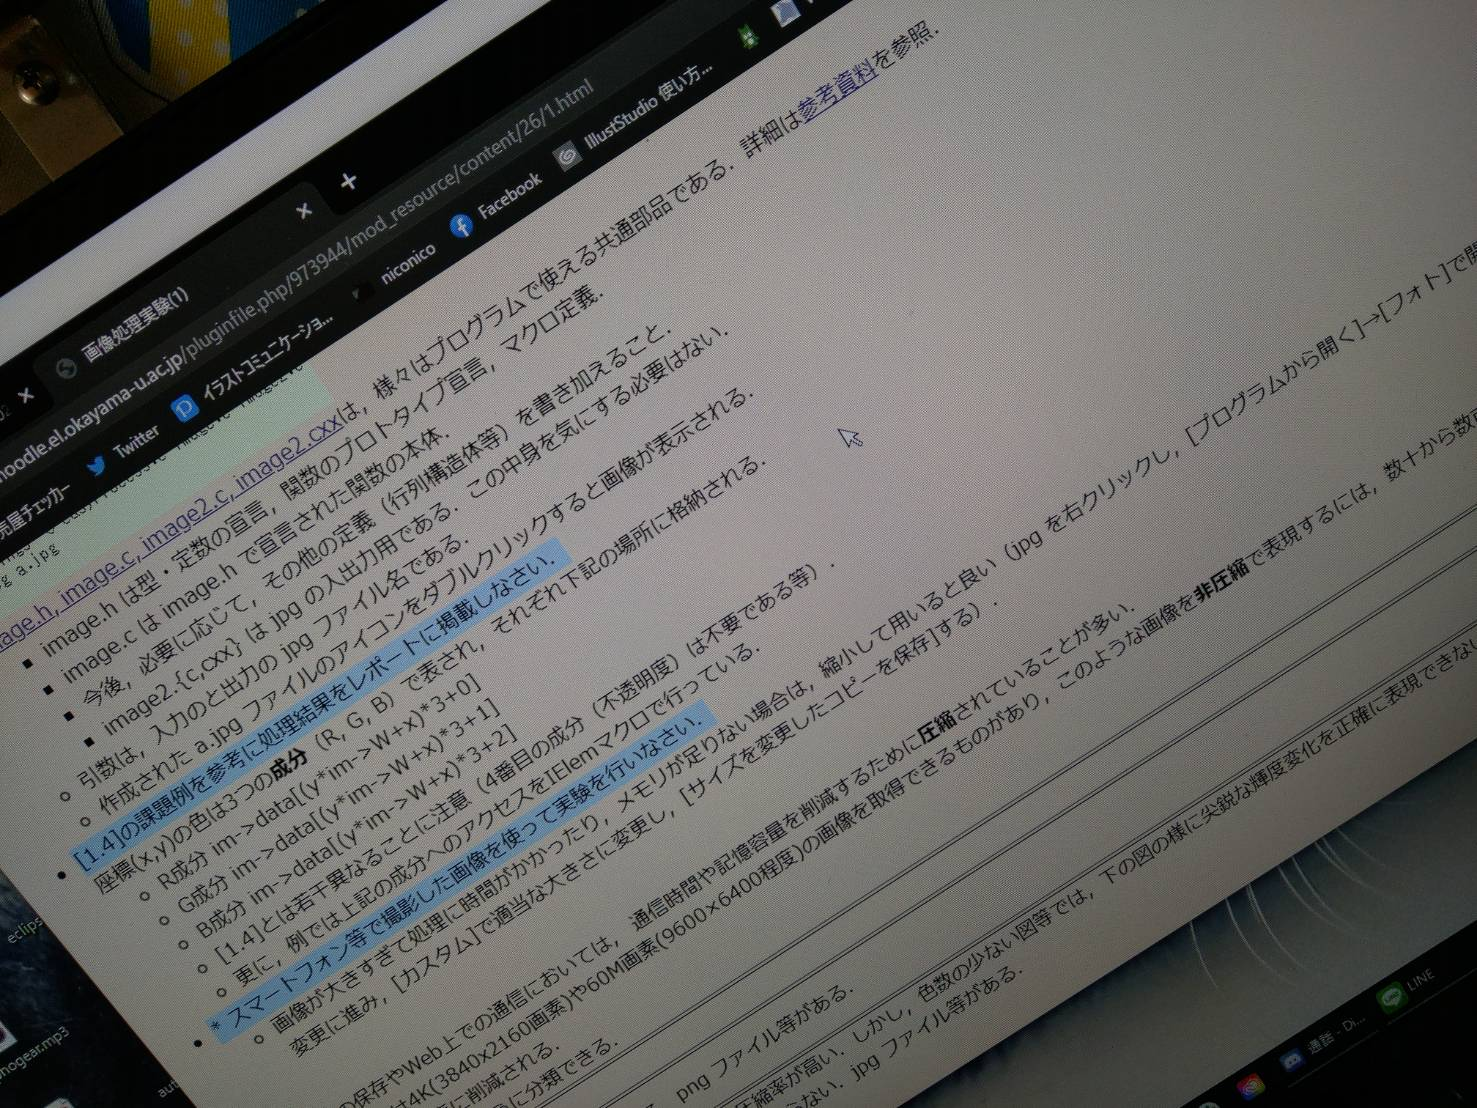
\includegraphics[scale=.1]{1-10.jpg}
    \caption{スマホで撮影した画像}
    \label{1-10.jpg}
\end{figure}

easyProcessで拡大について実験を行った.その結果は図\ref{1-11.jpg}に示した.
\begin{figure}[htbp]
    \centering
    
\includegraphics[scale=.1]{1-11.jpg}
    \caption{スマホで撮影した画像を拡大した結果}
    \label{1-11.jpg}
\end{figure}

\subsection{様々な型式でのファイルサイズ(および画質)を比較}

元形式がjpg形式の画像を用いて,png,gif,bmp,webpについてそれぞれ比較を行った.
画像の縦幅,横幅に変化はなく,純粋にファイルの書き出し形式のみ変更を行った.
\begin{table}[h]
    \begin{center}
    \begin{tabular}{l|llll}
    \cline{1-2}
    形式        & ファイルサイズ(B) &  &  &  \\ \cline{1-2}
    .jpg(元画像) & 7,692,612  &  &  &  \\
    .png      & 29,699,714 &  &  &  \\
    .gif      & 13,502,072 &  &  &  \\
    .bmp      & 36,578,442 &  &  &  \\
    .webp     & 7,192,510  &  &  &  \\ \cline{1-2}
    \end{tabular}
\end{center}
\end{table}

無圧縮であるWindows独自規格のbmpファイルについて見てみると,やはりファイルサイズは大きくなっている.
また,次いで可逆圧縮形式のpngのファイルサイズも大きくなっていた.Webなどではかなり使われている形式のため,
小さくなるかと思っていたがそうではなかった.
そして非可逆圧縮のgifは元画像の約2倍程度にまでファイルサイズが大きくなっている.
最後に,非可逆圧縮,可逆圧縮の両方を扱えるwebpについてだが,ここでは可逆圧縮で実験を行った.結果,jpgよりも500KB,少なくなった.

\section{画像の幾何学変換}

遠景を同一視点から撮影した画像を重ね合わせるには,射影変換を用いる.
射影変換は3x3行列で表されるため積によって変換の合成を行うことができる. なお,基本的な幾何学変換(回転・平行移動・拡大・縮小)は3行目が(0 0 1)の射影変換で表すことができる.

\subsection{(x,y)と(u,v)の位置に,ほぼ同じ物体が観測されていることを確認}
図\ref{2-1.png}からほぼ同じ物体が同じ位置に観測されている
\begin{figure}[h]
    \centering
    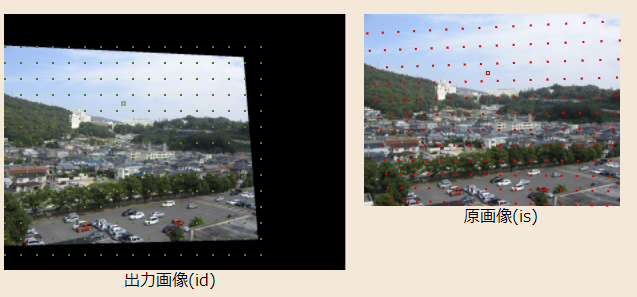
\includegraphics[scale=.5]{2-1.png}
    \caption{出力画像と元画像}
    \label{2-1.png}
\end{figure}

\subsection{射影変換 aの要素を変化させ画像の変化を確認}

\begin{verbatim}
    変更前の配列a
    a=[[ .866 , -.5  ,  160],
   [ .5   , .866 , -300],
   [-.001 , 0    ,    1]];

   変更後の配列a
   a=[[ .433 , -.5  ,  80],
   [ .5   , .433 , -150],
   [-.0001 , 0    ,    1]];
\end{verbatim}
\begin{figure}[h]
    \centering
    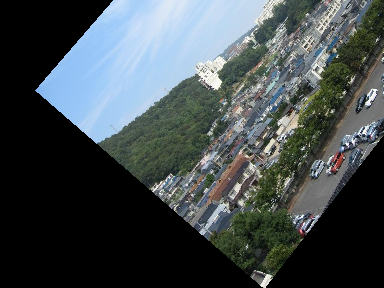
\includegraphics[scale=.5]{2-2.png}
    \caption{配列変更後の出力画像}
    \label{2-2.png}
\end{figure}

\subsection{C言語による実装例をもとに 上記と同様の処理を行う}
実装にあたり,ImageClear関数が定義されていなかったため,image.cにImageClear関数をまず定義した.
参考資料から,画像のすべての要素を黒で塗りつぶせば良いため,画像の画素数分ループ処理を行い,
全ての画素に黒の値である0を代入することで実装した.以下にそのソースを示す.
また結果は図\ref{2-3.jpg}に示した.

\begin{verbatim}
    void ImageClear(Image *im){
    for(int y=0;y<im->H;y++){
        for(int x=0;x<im->W;x++){
            IElem(im,x,y,0) = 0;
            IElem(im,x,y,1) = 0;
            IElem(im,x,y,2) = 0;
        }
    }
}
\end{verbatim}
\begin{figure}[h]
    \centering
    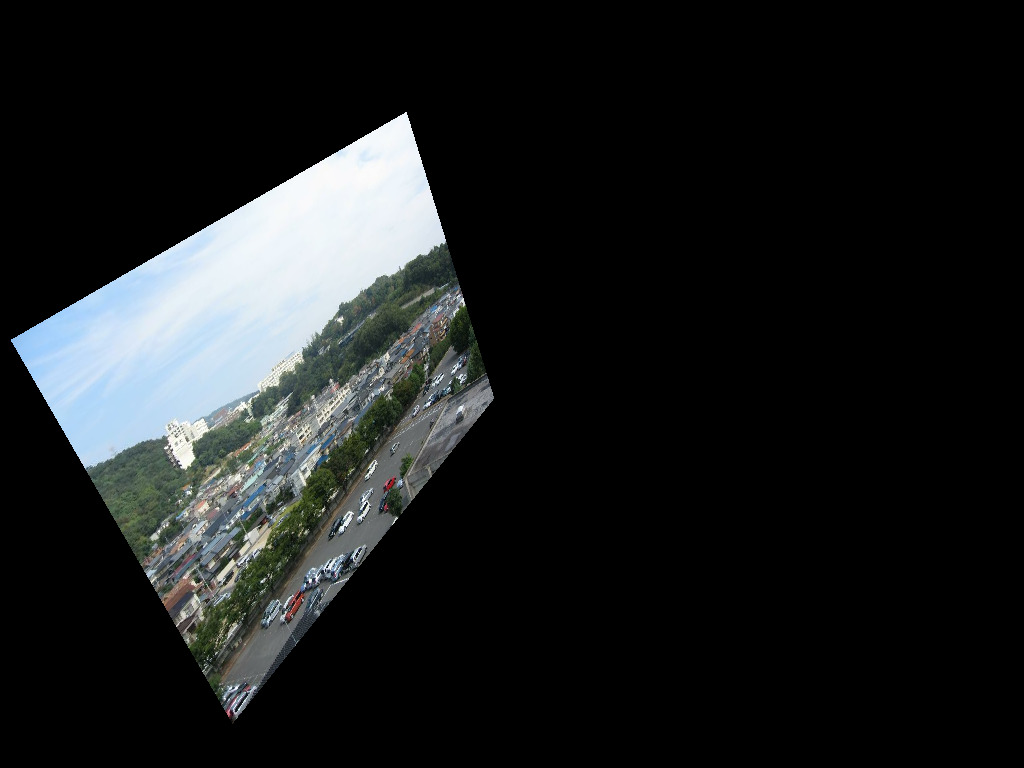
\includegraphics[scale=.15]{2-3.jpg}
    \caption{C言語による処理結果}
    \label{2-3.jpg}
\end{figure}

\subsection{m0d を適当な行列に変更しても,img1 と img0 の位置関係が保たれることを確認}
まず,図\ref{2-4.png}にm0d行列の変更前の画像を示す.
そして,次のように画像の全体の座標位置を右にずらすよう変更を加えたところ,図\ref{2-5.png}のような
結果が得られた.
この結果から,img1とimg0の位置関係はm0dを適当な行列に変更しても保たれていることが確認できた.
\begin{verbatim}
    var m0d=[[ 2.667,0,-500 ],
         [ 0,2.667,-100 ],
         [ 0,0,1 ]];
\end{verbatim}
\begin{figure}[htbp]
    \begin{tabular}{cc}
        \begin{minipage}{0.5\hsize}
            \begin{center}
                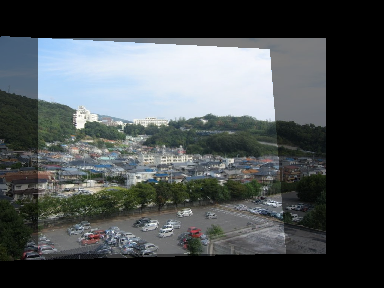
\includegraphics[scale=.5]{2-4.png}
                \caption{m0d行列変更前}
                \label{2-4.png}
            \end{center}
        \end{minipage}
        \begin{minipage}{0.5\hsize}
            \begin{center}
                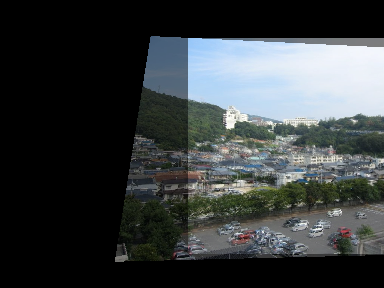
\includegraphics[scale=.5]{2-5.png}
                \caption{m0d行列変更後}
                \label{2-5.png}
            \end{center}
        \end{minipage}
    \end{tabular}
\end{figure}

\subsection{行列 m10 を修正し,ずれのない合成画像を作成することを試みる}
いくつかの行列を修正し,試みたがうまくずれをなくすことができなかった.

\subsection{m10 を算出し,合成に用いなさい}
実験のページに記載されているページの特徴点を動かすことで正しいm10を算出し,合成に用いた.
合成をしたい元画像の両方で特徴点が正確に同じ物体を指すようにするということを行い算出をした.
以下が算出した配列である.
なお,図\ref{2-6.png}が合成後の画像である.左下の部分をみると多少ブレが見られるものの多くの部分でブレがなくなっているためこの配列を回答とした.
\begin{verbatim}
    0.930421    0.018946    118.490952
    -0.043542   0.976597    22.193656
    -0.000097   0.000002    1.000000 
\end{verbatim}
\begin{figure}[h]
    \centering
    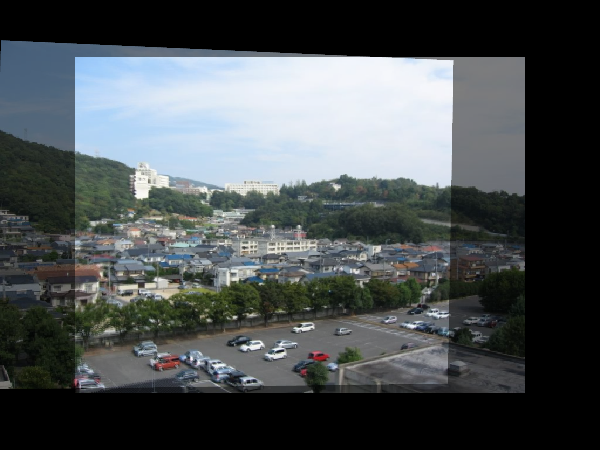
\includegraphics[scale=.5]{2-6.png}
    \caption{m10を修正した後の合成画像}
    \label{2-6.png}
\end{figure}

\subsection{3x3 行列の積を計算する関数 mult33 を実装し,m1d = m10 ˙ m0d を計算し,画像を合成}
3x3行列は,左の行列1行目の各要素を右側の行列1列目の各要素にかけて,それら3つの項を足しあわせ,1行1列要素
とする.左の行列1行目の各要素を右側の行列2列目の各要素にかけて・・・という手順を繰り返していき,3行3列要素目までを計算すればよい.

その実装としては,2重ループを用いて行った.左側は右側の3つ分が終わると次の行に進み,また,掛け合わす場所は定義より決まっているため,
以下のソースコードのようにした.
\begin{verbatim}
    void mult33(double d[3][3],double a[3][3],double b[3][3]){
    for(int i=0;i<3;i++){
        for(int j=0;j<3;j++){
            d[i][j] = a[i][0]*b[0][j] + a[i][1]*b[1][j] + a[i][2]*b[2][j]; 
        }
    }
}
\end{verbatim}
そして,これをpano0.cのmain関数にて使用したのが以下である.
ImageImageProjectionAlpha は,行列 m0d を使って im (0.jpg) を id に書き込む.m0dは結果を出力画像の中心寄りに表示するための平行移動
(右に100,下に100)を行う射影変換である.
行列 m1d を使った ImageImageProjectionAlpha は,id に im (1.jpg) を書き込む.m10 は img1 と img0 の関係を表し,m0d は img0 と 出力画像の関係を表す.
img1 と出力画像の関係は m10 と m0d の積で表される.このときに
パノラマ合成を行う必要があり,m10に,先程求めた算出後の配列を使用.また,m1dはm10とm0dの積で表されるため,
mult33を使い,積を計算した.パノラマ合成後の結果画像は図\ref{2-7.png}に示した.

\begin{verbatim}
    double m0d[][3]={
      1,0,-100,
      0,1,-100,
      0,0,1
    };
    im=ImageRead("0.jpg");
    ImageImageProjectionAlpha(id,im,m0d,.5);
    double m10[][3]={
      0.930421,   0.018946,   118.490952,
      -0.043542,  0.976597,   22.193656,
      -0.000097,  0.000002,   1.000000 
    }, m1d[3][3];
    mult33(m1d,m10,m0d);
\end{verbatim}

\begin{figure}[h]
    \centering
    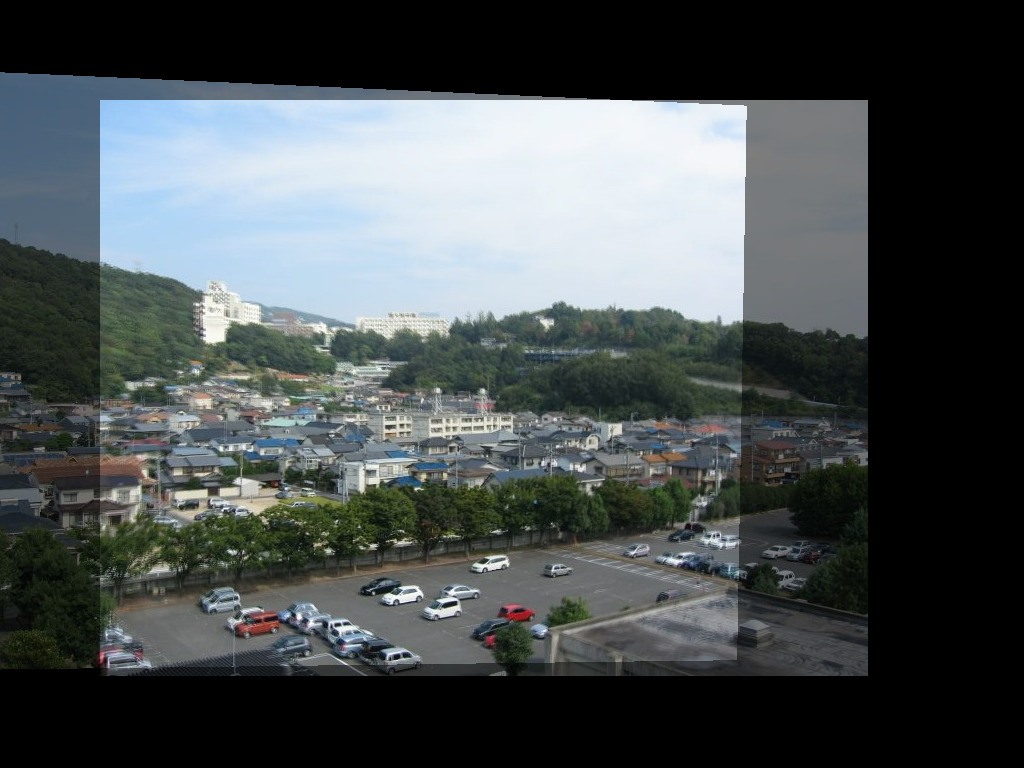
\includegraphics[scale=.3]{2-7.png}
    \caption{C言語でのパノラマ合成の結果画像}
    \label{2-7.png}
\end{figure}

\subsection{「原画像の座標(u,v)を出力画像の座標(x,y)に変換する行列」を A とすると,上記の実装で用いている a は A の逆行列である.}
これを確認するために,
    $ \left(
        \begin{array}{rrr}
        2 & 0 & 0 \\
        0 & 2 & 0 \\
        0 & 0 & 1
        \end{array}
    \right) $
の,逆行列
$ \left(
    \begin{array}{rrr}
    0.5 & 0 & 0 \\
    0 & 0.5 & 0 \\
    0 & 0 & 1
    \end{array}
\right) $
をかけたときに2倍になるかどうかを見る.

homography.cの配列aを先程の逆行列のように変え,実行すると図\ref{2-8.jpg}のようになった.
\begin{figure}[h]
    \centering
    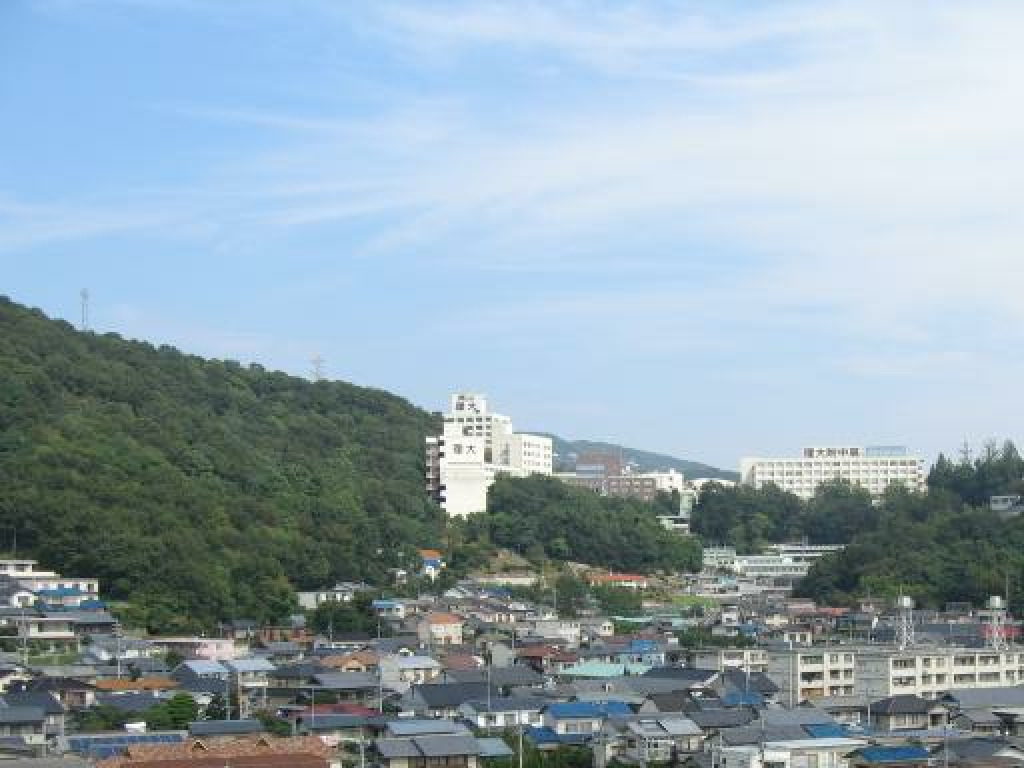
\includegraphics[scale=.2]{2-8.jpg}
    \caption{結果}
    \label{2-8.jpg}
\end{figure}

きちんと拡大されていたことが確認できた.

\section{変換行列の算出}
\subsection{1.jpg を 0.jpg に重ねる3x3行列m10の計算法の詳細の手順の確認}
初期状態が以下の表を確認する.この動作は行列 $A^{T}$($Q^{T}$), R, ベクトル $b^{T}$, $tmp^{T}$という操作で,45回実行することで,4組の対応点の座標から射影変換行列が計算される.
\tiny
\begin{verbatim}
    initialized
     256.000000        0.000000      347.000000        0.000000      263.000000        0.000000      413.000000        0.000000 
     218.000000        0.000000      220.000000        0.000000      367.000000        0.000000      315.000000        0.000000 
       1.000000        0.000000        1.000000        0.000000        1.000000        0.000000        1.000000        0.000000 
       0.000000      256.000000        0.000000      347.000000        0.000000      263.000000        0.000000      413.000000 
       0.000000      218.000000        0.000000      220.000000        0.000000      367.000000        0.000000      315.000000 
       0.000000        1.000000        0.000000        1.000000        0.000000        1.000000        0.000000        1.000000 
  -94976.000000   -58880.000000  -160661.000000   -79810.000000  -100729.000000   -99677.000000  -218890.000000  -135051.000000 
  -80878.000000   -50140.000000  -101860.000000   -50600.000000  -140561.000000  -139093.000000  -166950.000000  -103005.000000 

       0.000000        0.000000        0.000000        0.000000        0.000000        0.000000        0.000000        0.000000 
       0.000000        0.000000        0.000000        0.000000        0.000000        0.000000        0.000000        0.000000 
       0.000000        0.000000        0.000000        0.000000        0.000000        0.000000        0.000000        0.000000 
       0.000000        0.000000        0.000000        0.000000        0.000000        0.000000        0.000000        0.000000 
       0.000000        0.000000        0.000000        0.000000        0.000000        0.000000        0.000000        0.000000 
       0.000000        0.000000        0.000000        0.000000        0.000000        0.000000        0.000000        0.000000 
       0.000000        0.000000        0.000000        0.000000        0.000000        0.000000        0.000000        0.000000 
       0.000000        0.000000        0.000000        0.000000        0.000000        0.000000        0.000000        0.000000 

     371.000000      230.000000      463.000000      230.000000      383.000000      379.000000      530.000000      327.000000 

       0.000000        0.000000        0.000000        0.000000        0.000000        0.000000        0.000000        0.000000 
\end{verbatim}
\normalsize
45回実行後の行列が以下のようであった.
\tiny
\begin{verbatim}
    done
       0.392371        0.000000        0.531847        0.000000        0.403100        0.000000        0.633005        0.000000 
       0.013540        0.000000       -0.437106        0.000000        0.876890        0.000000       -0.199546        0.000000 
       0.746709        0.000000        0.224407        0.000000       -0.041838        0.000000       -0.624754        0.000000 
       0.000000        0.392371        0.000000        0.531847        0.000000        0.403100        0.000000        0.633005 
       0.000000        0.013540        0.000000       -0.437106        0.000000        0.876890        0.000000       -0.199546 
       0.000000        0.746709        0.000000        0.224407        0.000000       -0.041838        0.000000       -0.624754 
      -0.295032       -0.448602        0.378993        0.576267        0.142043        0.215980       -0.226004       -0.343644 
      -0.448602        0.295032        0.576267       -0.378993        0.215980       -0.142043       -0.343644        0.226004 

     652.443867      549.877189        1.960322        0.000000        0.000000        0.000000  -301875.042231  -248248.300143 
       0.000000      165.750042        0.253778        0.000000        0.000000        0.000000    24290.303105   -46513.794686 
       0.000000        0.000000        0.304524        0.000000        0.000000        0.000000    33993.758735    26933.037130 
       0.000000        0.000000        0.000000      652.443867      549.877189        1.960322  -191217.160969  -167855.917552 
       0.000000        0.000000        0.000000        0.000000      165.750042        0.253778   -26368.674762   -79976.364619 
       0.000000        0.000000        0.000000        0.000000        0.000000        0.304524    26667.777043    21377.198091 
       0.000000        0.000000        0.000000        0.000000        0.000000        0.000000     7596.900540     1712.683064 
       0.000000        0.000000        0.000000        0.000000        0.000000        0.000000        0.000000     5458.391125 

     371.000000      230.000000      463.000000      230.000000      383.000000      379.000000      530.000000      327.000000 

       0.980063        0.155844       98.500361       -0.055756        1.153389        0.503900       -0.000139        0.000316 
\end{verbatim}
\normalsize

\subsection{C言語による実装例}
講義ページ内のC言語による実装のファイルを編集した.具体的には,MatrixQRDecompColMajor関数と
MatrixSimeqLr関数を書き換えた.この2つの関数には,8行8列分の操作はなかったため,すでに記載してある手続きと,資料のPDFの4組の場合の射影変換行列を参考に実装をした.

まず,MatrixQRDecompColMajorは,資料のPDF内の式(12)からの処理を行う. なお,実装例の配列aTが3行分しか用意されいていないが,実際には8行分必要であることに注意して,以下のように8行分宣言を行った.
\begin{verbatim}
  double *aT[] = {  Row(mt,0), Row(mt,1), Row(mt,2), Row(mt,3), Row(mt,4), 
                    Row(mt,5), Row(mt,6), Row(mt,7) } ;
\end{verbatim}
次のようなAの各列を$a_{i}$と表した行列
\begin{equation}
  A \colon = [a_{0}, a_{1}...], R \colon = (r_{ij})
\end{equation}

行列は,資料のPDFの式(12)から式(21)によりQに書き換えられ,積QRはもとのAと等しくなる.
具体的な動作手順としては,$a_0$の場合,単位ベクトルへの変換.$a_1$の場合,1回の直交化と単位ベクトルの変換.
$a_2$の場合,2回の直交化のための動作と単位ベクトルへの変換というように規則に沿ったものになっている.
なお,この過程で,Rの要素も得られており,式 (12), 式 (14), 式 (17) 等の分母が対角項$r_{ii}$,式 (13),
式 (15), 式 (16) 等の内積 ($a^{T}_{i}$ $a_j$ ) が非対角項 $r_{ij}$ である.
その実装のソースを一部抜粋したのを以下で示す.

\begin{verbatim}
   Elem(mtR,0,0) = t = sqrt(VP(aT[0],aT[0],W));
   VSS(aT[0], 1/t, W);

 ///////////
   Elem(mtR,0,1) = t = VP(aT[0], aT[1], W);
   VSA(aT[1], aT[0], -t, W);

   Elem(mtR,1,1) = t = sqrt(VP(aT[1],aT[1],W));
   VSS(aT[1], 1/t, W);

 ///////////
   Elem(mtR,0,2) = t = VP(aT[0], aT[2], W);
   VSA(aT[2], aT[0], -t, W);

   Elem(mtR,1,2) = t = VP(aT[1], aT[2], W);
   VSA(aT[2], aT[1], -t, W);

   Elem(mtR,2,2) = t = sqrt(VP(aT[2],aT[2],W));
   VSS(aT[2], 1/t, W);
\end{verbatim}

次に,MatrixSimeqLrはPDF内の式(22)の後ろに書いてある後退代入を行う.
上三角行列で有ることに注意する.
\begin{eqnarray}
  x_2 = t_2 / r_{22}\\
  x_1 = (t_1 - x_2 r_12)/r_{11}\\
  x_0 = (t_0 - \sum_{i=1}^{2} x_i r_{0i})/r_{00}
\end{eqnarray}
目的の解がi個なら,$x_{i}$のiが小さくなるにつれ,引いていく要素が多くなる.
3x3の例を参考に,8x8の実装したもののソースコードの一部を抜粋したものを示す.

\begin{verbatim}
  B[7] =  B[7] / Elem(mtR,7,7);
  B[6] = (B[6]-B[7]*Elem(mtR,6,7)) / Elem(mtR,6,6);
  B[5] = (B[5]-B[6]*Elem(mtR,5,6)-B[7]*Elem(mtR,5,7)) / Elem(mtR,5,5);
  B[4] = (B[4]-B[5]*Elem(mtR,4,5)-B[6]*Elem(mtR,4,6)-B[7]*Elem(mtR,4,7)) / Elem(mtR,4,4);
\end{verbatim}

これを実装し,実際に出力された画像を図\ref{3-1.jpg}に示す.

\begin{figure}[ht]
  \centering
  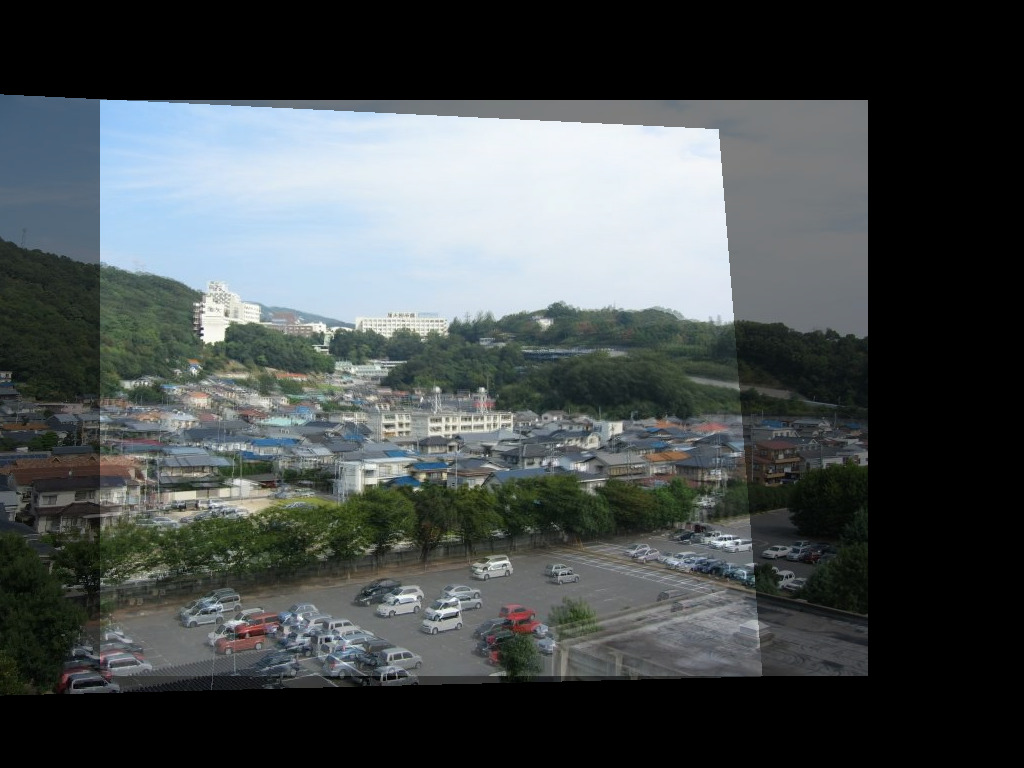
\includegraphics[scale=.2]{3-1.jpg}
  \caption{実際に出力された画像}
  \label{3-1.jpg}
\end{figure}

\subsection{どのような大きさの行列でも扱えるように,ループを用いて実装}

まず,MatrixQRDecompColMajorの配列の個数を動的に確保することから始めた.
\begin{verbatim}
  double **aT = (double **)malloc((sizeof (double *)) * mt->H);
\end{verbatim}
配列の確保はmallocでポインタのポインタaTと宣言することで,後の処理で配列のように扱える.
double **aTという宣言は,ポインタaTが示す先もポインタ*aTであり,そのポインタ*aTという宣言は,ポインタaTが示す先もポインタ
**aTであるということである.
その状態で,mallocにより,double *ポインタを目的の要素分宣言することで,配列要素aT[mt->H]分
求めることができる.この配列aT[0],aT[1]...はポインタであり,その示す先の*at[0],*aT[1]...は
double型であり,ポインタの配列を宣言することになる.その後,aT[0]からaT[mt->H]までの
各要素にRowを格納することでmt->Hがいくらであっても確保できる.

\begin{verbatim}
  double **aT = (double **)malloc((sizeof (double *)) * mt->H);
  //縦に伸びていく 
  for(int get=0; get<mt->H;get++){
      aT[get] = Row(mt,get);
  }
\end{verbatim}


そして,その後のシュミットの直交化手順だが,二重ループを用いた.
確保した要素分(W個分)のaT[i]について手続きを施す.iが増えるに連れ,行うVSA(ベクトルのスカラ倍加算)の回数も増えることに
注意すると,その回数はiを超えない回数行う事となる.
そして,jとiが同じ時にベクトルを単位ベクトルにする動作をする.

以下がそのソースコードである.
\begin{verbatim}
  for(int i=0; i < W; i++){
    for(int j=0; j <= i; j++){
        // printf("%d,%d\n",i,j);
        if(j == i){
            Elem(mtR,j,i) = t = sqrt(VP(aT[j],aT[i],W));
            VSS(aT[i], 1/t, W);
        }else{
            Elem(mtR,j,i) = t = VP(aT[j], aT[i], W);
            VSA(aT[i], aT[j], -t, W);
        }
    }
}
\end{verbatim}

もう一つ,MatrixSimeqLrについて.要素数は,mtR->Wにより可変的に行うことができる.
ここで,8x8の場合を考えてみる.配列の要素数は0~7の8個である.
B[7]の場合,自身をElem(mtR,7,7)で割る動作のみ,B[6]の場合,自身からB[7]にElem(mtR,6,7)をかけたものを引き,Elem(mtR,6,6)で割る.
B[5]の場合,自身からB[6]にElem(mtR,5,6)をかけたものを引き,B[7]にElem(mtR,5,7)をかけたものを引き,Elem(mtR,6,6)で割るという手続きが続く.
これを2重ループに落とし込むと,大きいループの回数は,要素数個分繰り返す.今回は,iの大きい順から手続きを施した.
一度初回を飛ばし,2回目のループであるi=6のときについて考えると,i+1 = 7で一つ大きい添字の要素を参照でき,$\sum$ と同等の処理を内部のループで行える.
$\sum$のくりかえし最大回数は,要素数個分であるから,mtR-\verb|>|W = 8 つまり,配列の添字7までである.
その後,Elemで割るという動作を行えば良い.
では初回のi=7の時を見てみる.一つ添字の大きい要素は8だが,内部の$\sum$にあたるループの上限7を超えているのでループは実行されず,
自身をElemで割るという動作のみ行われることになる.

以下そのソースコードである.
\begin{verbatim}
  for(int i=mtR->W-1; 0<=i; i--){
    for(int j=i+1; j<mtR->W; j++){
      B[i] -=  B[j]*Elem(mtR,i,j);
    }
    B[i] = B[i] / Elem(mtR,i,i);
  }
\end{verbatim}

実行したところ,図\ref{3-1.jpg}と同じ結果が得られた.

\subsection{合成画像の品質を改善}
元々示されていた特徴点は,
\begin{verbatim}
  256,218,  371,230,
  347,220,  463,230,
  263,367,  383,379,
  413,315,  530,327,
\end{verbatim}
だが,出力された画像は図\ref{3-1.jpg}であり,あまり精度がよくない.
それを以下のように変更し,なるべく特徴点同士が離れるようにした.
\begin{verbatim}
  147,535,268,544,
  116,209,235,224,
  509,205,629,210,
  432,517,550,530
\end{verbatim}

それにより実行した結果が図\ref{3-2.jpg}である.少し粗はあるものの,図\ref{3-2.jpg}と比べると大きく改善しただろう.
\begin{figure}[ht]
\centering
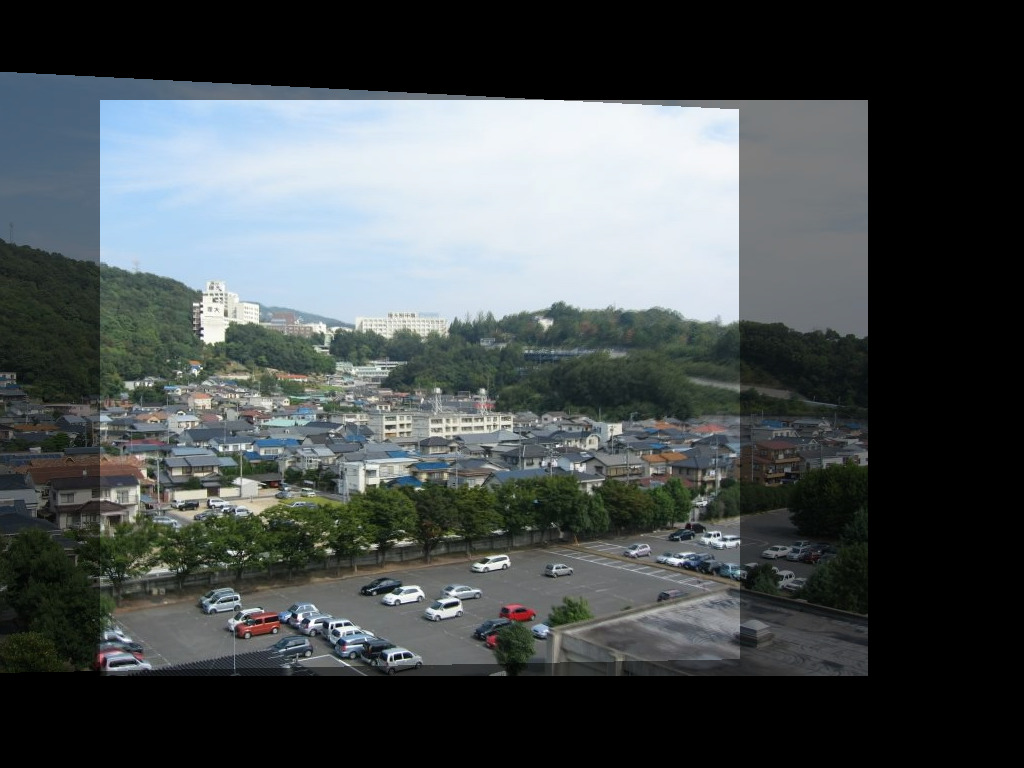
\includegraphics[scale=.3]{3-2.jpg}
\caption{特徴点の改善後}
\label{3-2.jpg}
\end{figure}

\subsection{自分で撮影した画像を合成}
撮影した画像がとても大きいサイズだったため,実験同様768x576までサイズを落として実行した.
合成に用いた画像は,図\ref{3-3.jpg},図\ref{3-4.jpg}である.
正確に同じ視点を撮ることができなかったため,真横に100px分だけ移動した画像になっている
特徴点は,以下のように設定した.
\begin{verbatim}
  215,320,  315,319,
  220,507,  320,506,
  651,480,  751,479,
  600,135,  700,134
\end{verbatim}

\begin{figure}[ht]
  \begin{minipage}{0.5\hsize}
    \centering
    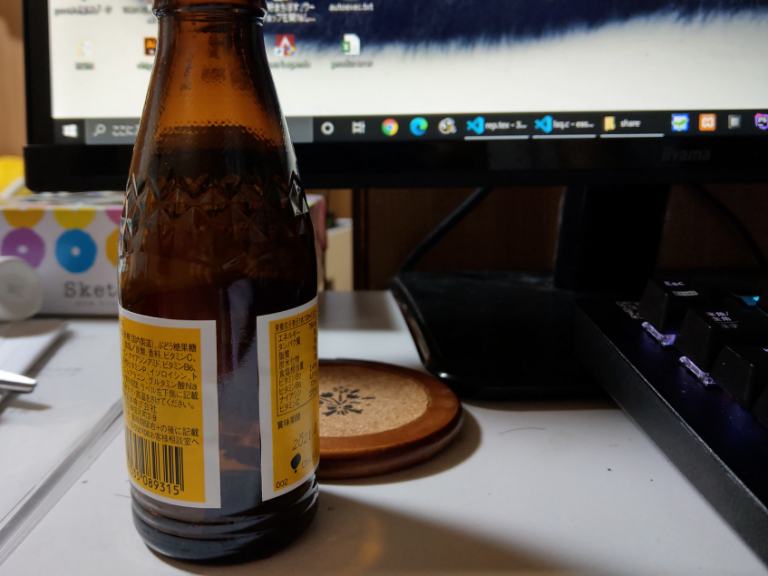
\includegraphics[scale=.3]{3-3.jpg}
    \caption{合成1枚目}
    \label{3-3.jpg}
  \end{minipage}
  \begin{minipage}{0.5\hsize}
    \centering
    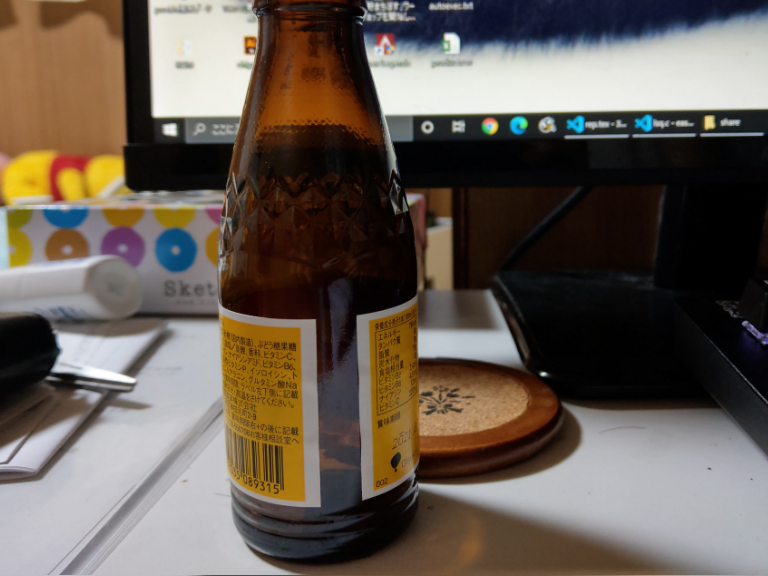
\includegraphics[scale=.3]{3-4.jpg}
    \caption{合成2枚目}
    \label{3-4.jpg}
  \end{minipage}
\end{figure}

プログラムを実行すると,図\ref{3-5.jpg}のようなパノラマ画像が合成された.
\begin{figure}[t]
    \centering
    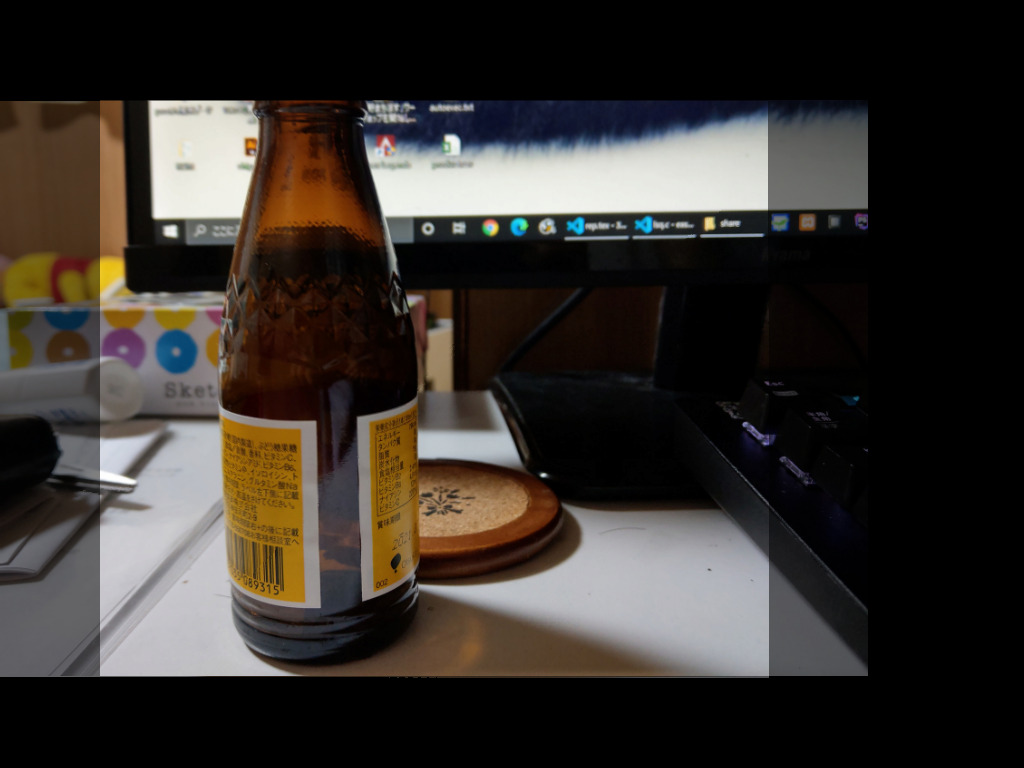
\includegraphics[scale=.5]{3-5.jpg}
    \caption{自分で撮影した画像のパノラマ}
    \label{3-5.jpg}
\end{figure}

\section{特徴点の自動検出}
画像合成の自動化には,特徴点の自動検出と自動対応付けが必要である.
これは,次のように2段階で行う.各画素が特徴点としてふさわしいかどうかを測る指標を計算する(第4回の課題).それが極大となる点を探し出す(第5回の課題).これらの計算の主要部分は,畳み込みフィルタである(ある点の出力値はその周辺の入力値の線形和で計算される).畳み込みフィルタは計算量が多いが,並列性が高いためGPUやマルチコアCPUによって効率的に計算できる.

\subsection{cpuで「特徴点らしさ」画像を出力}

資料の例を元に実装を完成させた.DElem,Elemがimage.hに定義されていなかったので,第3回および第2回を元に移植させた.
そして,Matrix構造体\verb|Matrix *MatrixAlloc|についても移植をおこなった.

最後に,今回の要であるImageFeature関数についてだが,iyに関する計算.そして,iyy,ixxの$\sum$に相当する
計算を行う処理を加えた.以下がその部分のソースコードである.
\begin{verbatim}
    ix = IElem(im, x+u+1, y+v, 1) - IElem(im, x+u-1, y+v, 1);
    iy = IElem(im, x+u, y+v+1, 1) - IElem(im, x+u, y+v-1, 1);
    ixx += ix*ix; // ixx だけでなく ixy,iyy も計算する. 
    iyy += iy*iy;
    ixy += ix*iy;
\end{verbatim}
さらに,DElemには行列
\[
  \left(
    \begin{array}{cc}
      i_{xx} & i_{xy} \\
      i_{xy} & i_{yy} \\
    \end{array}
  \right)
\]
の小さい方の固有値を入れることで求める事ができるが,
2行2列の行列の固有値は2次方程式の解の公式で求めることと同じであるため
解の公式を使った.

\begin{verbatim}
    DElem(im2,x,y) = 
    ((ixx + iyy)-sqrt(pow(ixx+iyy,2.0)-4.0*(ixx*iyy-ixy*ixy)))/2.0;
\end{verbatim}
Wで,自分の周りの上下左右の7マスを見て特徴点を取っている.
この実装で出力された結果は図\ref{4-1.jpg}に示した.このときのWは7である.
処理時間は3.9GhzのCPUで144msecだった.

\begin{figure}[t]
    \centering
    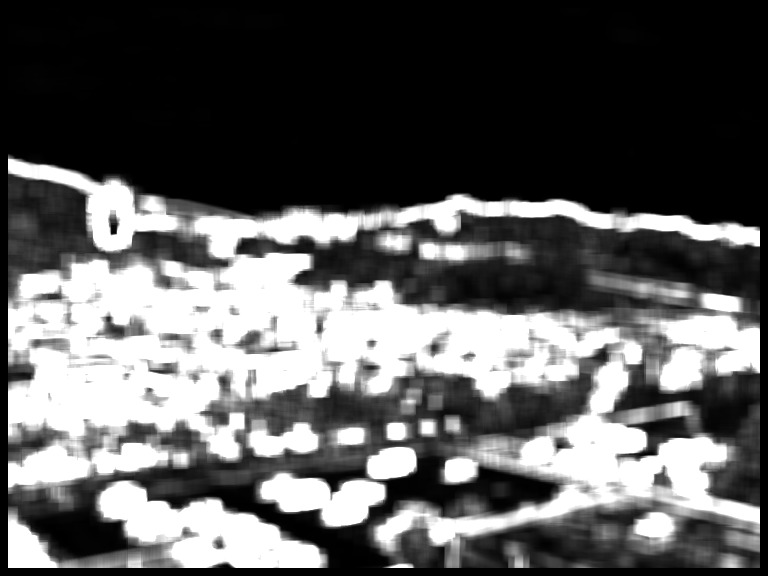
\includegraphics[scale=.5]{4-1.jpg}
    \caption{出力結果}
    \label{4-1.jpg}
\end{figure}

\subsection{CPUでの分解}
資料を元に,3重ループを2回行うことで実装した.
資料には,
特徴点検出のixx,ixy,iyyは15x15の平滑化であり225個の和である.
これを直接計算するより,横に隣接する15画素の和を中間配列に格納し,
この配列の縦15要素の和によって最終結果を計算するとあるので,それを再現するようにした.
出力結果は図\ref{4-2.jpg}に示す.計算時間は36msecであった.
\begin{verbatim}
        int x,y,u,v,ix,iy;
        for(y=1;y<im->H-1;y++) for(x=W+1;x<im->W-W-1;x++){
              double ixx,ixy,iyy;
              ixx=iyy=ixy=0;
              for(u=-W;u<=W;u++){
                ix = IElem(im, x+u+1, y, 1) - IElem(im, x+u-1, y, 1);
                iy = IElem(im, x+u, y+1, 1) - IElem(im, x+u, y-1, 1);
                ixx += ix*ix;
                iyy += iy*iy;
                ixy += ix*iy;
          }
          DElem(im3,x,y) = ixx;
          DElem(im4,x,y) = ixy;
          DElem(im5,x,y) = iyy;
        }
          for(y=W+1;y<im->H-W-1;y++) for(x=W+1;x<im->W-W-1;x++){
              double ixx,ixy,iyy;
              ixx=iyy=ixy=0;
              for(v=-W;v<=W;v++){
                ixx += DElem(im3, x, y+v);
                ixy += DElem(im4, x, y+v);
                iyy += DElem(im5, x, y+v);
          }
          DElem(im2,x,y) = 
          ((ixx + iyy)+sqrt(pow(ixx+iyy,2.0)-4.0*(ixx*iyy-ixy*ixy)))/2.0;
        }
\end{verbatim}
\begin{figure}[t]
    \centering
    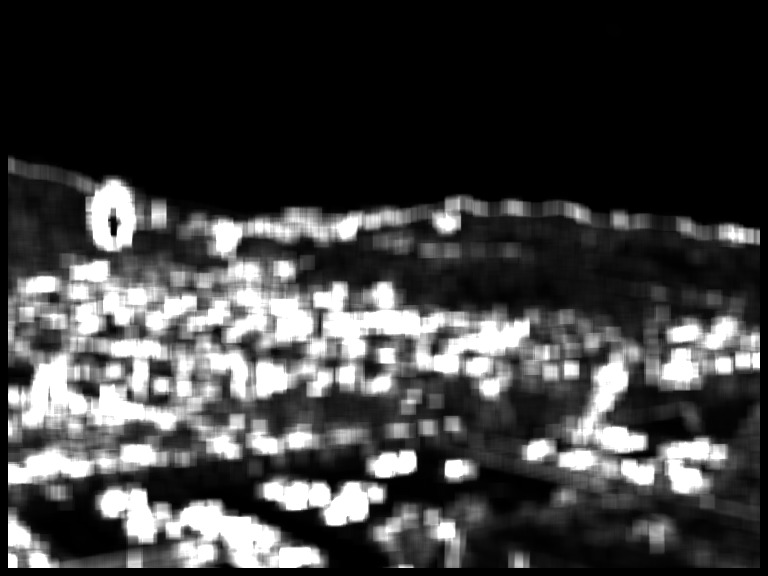
\includegraphics[scale=.5]{4-2.jpg}
    \caption{出力結果}
    \label{4-2.jpg}
\end{figure}

\subsection{実行時間の比較}
CPUとCPU分解の2つの時間を示す.
\begin{table}[h]
    \centering
    \begin{tabular}{l|llll}
    \cline{1-2}
    方法    & 時間(msec) &  &  &  \\ \cline{1-2}
    CPU   & 144      &  &  &  \\
    CPU分解 & 34       &  &  &  \\ \cline{1-2}
    \end{tabular}
    \end{table}

\subsection{自分で撮影した画像で実験}
作成したCプログラムに,図\ref{4-3.jpg}を与えて出力された結果を図\ref{4-4.jpg}に示した.

\begin{figure}[h]
    \begin{minipage}{0.5\hsize}
        \centering
        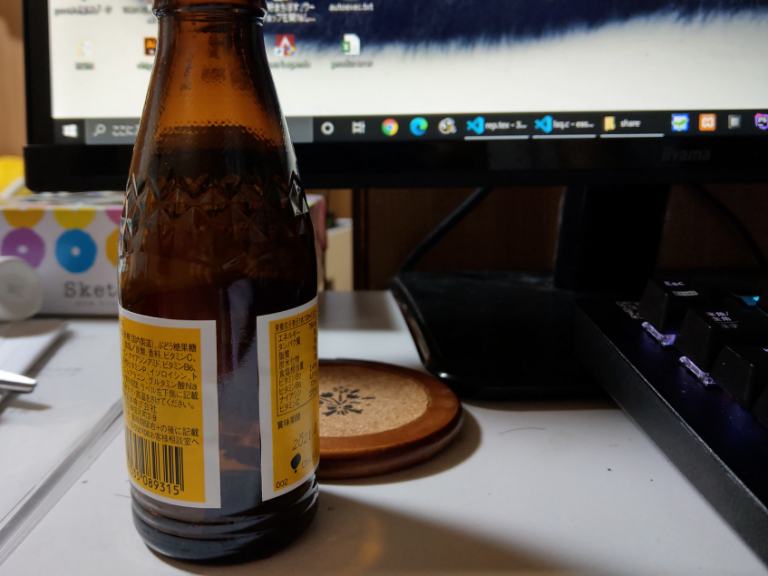
\includegraphics[scale=.3]{4-3.jpg}
        \caption{元画像}
        \label{4-3.jpg}
    \end{minipage}
    \begin{minipage}{0.5\hsize}
        \centering
        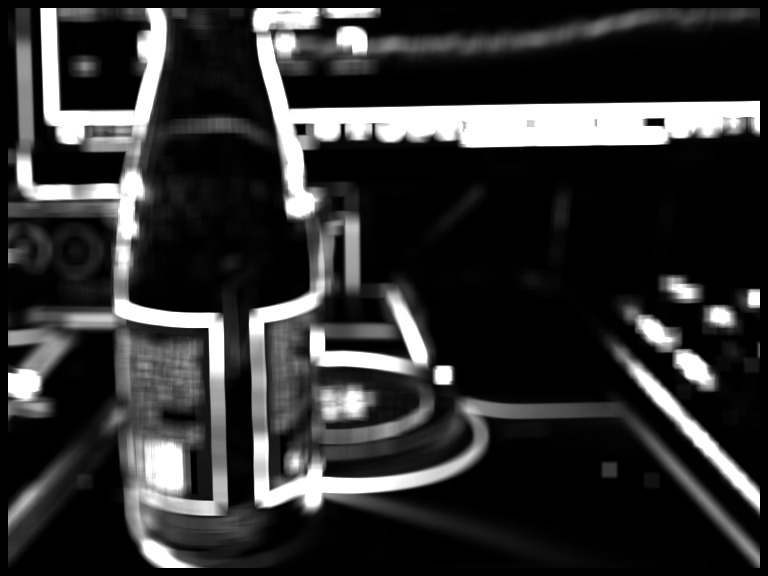
\includegraphics[scale=.3]{4-4.jpg}
        \caption{出力結果}
        \label{4-4.jpg}
    \end{minipage}
\end{figure}

\subsection{Wの値をコマンドラインから指定}

まず,image.hのImageDrowBoxの宣言にWを整数型で追加した.
そして,使用する際にコマンドライン引数をatoiを使い,整数型に変えることで対応した.
\begin{verbatim}
    ImageDrawBox(im,kk[i][0],kk[i][1],atoi(av[2]));
\end{verbatim}

\subsection{Wの値を変えて複数回実行}
wの値を0から10まで変えて画像の出力をした.数字が大きくなるにつれて処理時間も増えていった.
その出力結果を数枚添付する.W=2からW=4あたりが綺麗に輪郭が出ている.
W=7以上は輪郭が太くなりすぎてあまり綺麗でなかった.
\begin{figure}[h]
    \begin{minipage}{0.5\hsize}
        \centering
        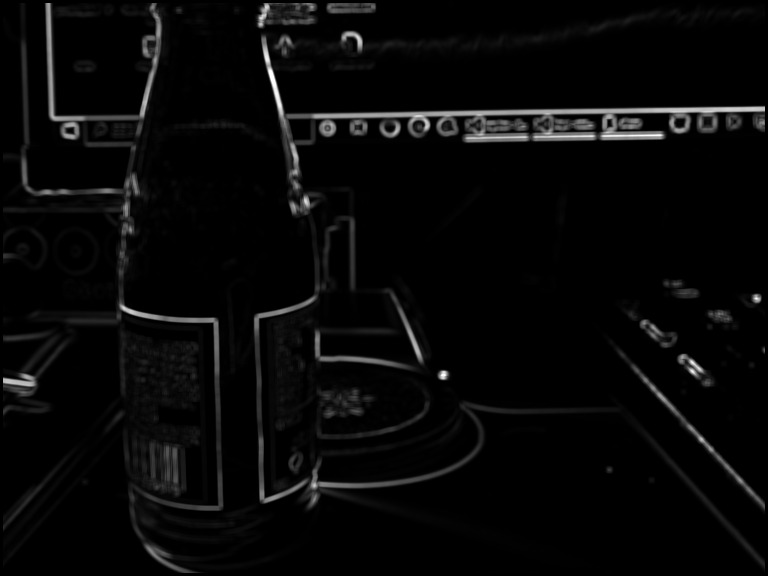
\includegraphics[scale=.3]{w2.jpg}
        \caption{W=2}
    \end{minipage}
    \begin{minipage}{0.5\hsize}
        \centering
        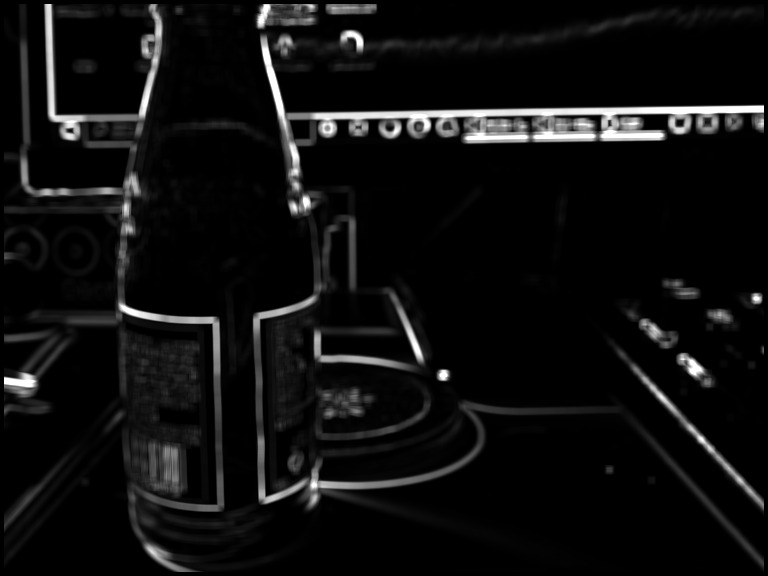
\includegraphics[scale=.3]{w3.jpg}
        \caption{W=3}
    \end{minipage}
\end{figure}
\begin{figure}[h]
    \begin{minipage}{0.5\hsize}
        \centering
        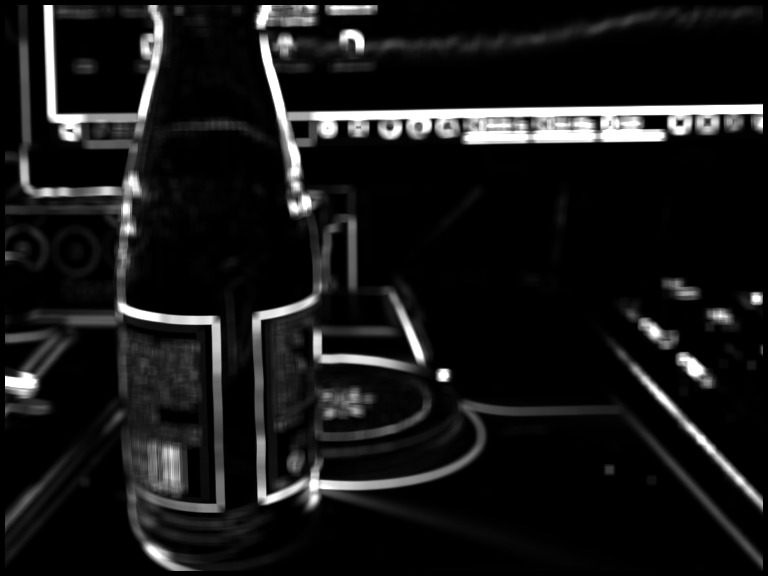
\includegraphics[scale=.3]{w4.jpg}
        \caption{W=4}
    \end{minipage}
    \begin{minipage}{0.5\hsize}
        \centering
        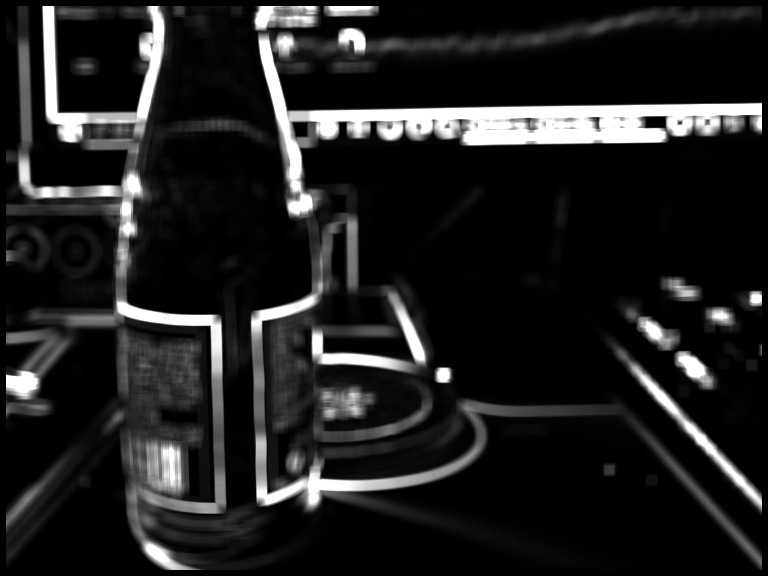
\includegraphics[scale=.3]{w5.jpg}
        \caption{W=5}
    \end{minipage}
\end{figure}
\begin{figure}[h]
    \begin{minipage}{0.5\hsize}
        \centering
        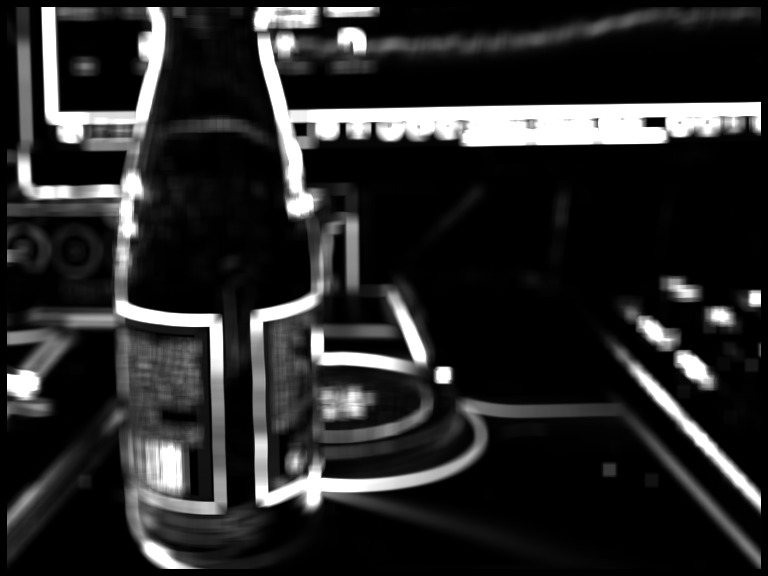
\includegraphics[scale=.3]{w6.jpg}
        \caption{W=6}
    \end{minipage}
    \begin{minipage}{0.5\hsize}
        \centering
        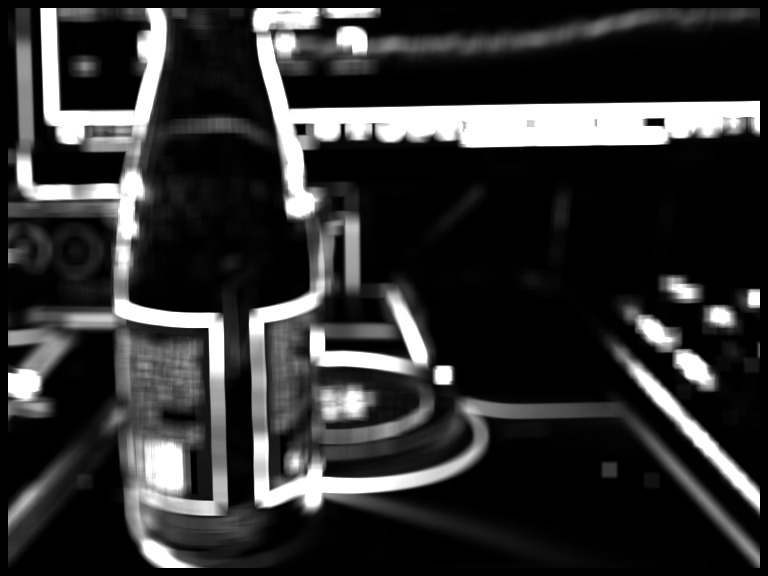
\includegraphics[scale=.3]{w7.jpg}
        \caption{W=7}
    \end{minipage}
\end{figure}

\section{特徴点の自動検出 2}
特徴点指標画像の極大点を検出する.
極大の判定は容易に並列実行できるが,極大の記録は並列的ではないため注意が必要である.前項で得られた極大点は,周辺よりは特徴的だが,画像全体で特徴的であるとは限らない.そこで,検出された点から画像全体で特徴的な点を選び出す.結果は図\ref{5-1.jpg}と図\ref{5-2.jpg}に示した.

\subsection{極大値を探し出し,その座標を配列に記録する部分を完成}

外側の2重ループで,x方向とy方向の走査をしている.
中身でWに対応する短形領域内での最大値を探す.Wはコマンドライン引数から与えることができる.
このとき,Wの値が小さすぎると,点が出てこずにセグメンテーションフォールトが起きてしまう.

そして,最大値が操作している点と同じならそこを特徴点として記録している.以下そのソースコードである.

\begin{verbatim}
    for(y=W+1;y<im2->H-W-1;y++){
        for(x=W+1;x<im2->W-W-1;x++){
          double max=-1;
          for(v=-W;v<=W;v++){
            for(u=-W;u<=W;u++){
              // (x,y) を中心とする 15x15 の矩形領域内で DElem(im2,x+u,y+v) の最大値を探す.
              if(DElem(im2, x+u, y+v) > max){
                max = DElem(im2,x+u,y+v);
              } 
            }
          }
          // 最大値が DElem(im2,x,y) と等しいなら,(x,y) を特徴点として記録する. 
          if(max == DElem(im2,x,y)){
            a = n++; 
            w[a][0] = x;
            w[a][1] = y;
            w[a][2] = max;
          }
        }
      }
\end{verbatim}

\subsection{得られた極大点リストから,「特徴点らしさ」の大きいものを N 個選び出す}

ここでは,qsort関数を用いてソートをした.

\begin{verbatim}
    qsort(kk, kw, sizeof(kk[0]),desc);
\end{verbatim}

kkは予め宣言されている配列で,kwはMatrixLocalMaxの返り値として赤い点の個数が与えられている.要素の1つ分はx,y,maxについて3つ分あるのでkk[0]で記載.
descという関数は降順に並び替えるものである.
\begin{verbatim}
    int desc(int left[3], int right[3])
    {
      return right[2]-left[2];
    }
\end{verbatim}

出力された点を一部抜粋すると,maxの値で降順に並んでいる.
\begin{verbatim}
    383 465 790611
    614 440 755117
    354 500 745975
    403 462 714745
    242 528 701629
    295 498 656782
    687 482 626184
\end{verbatim}

\begin{figure}[ht]
  \centering
  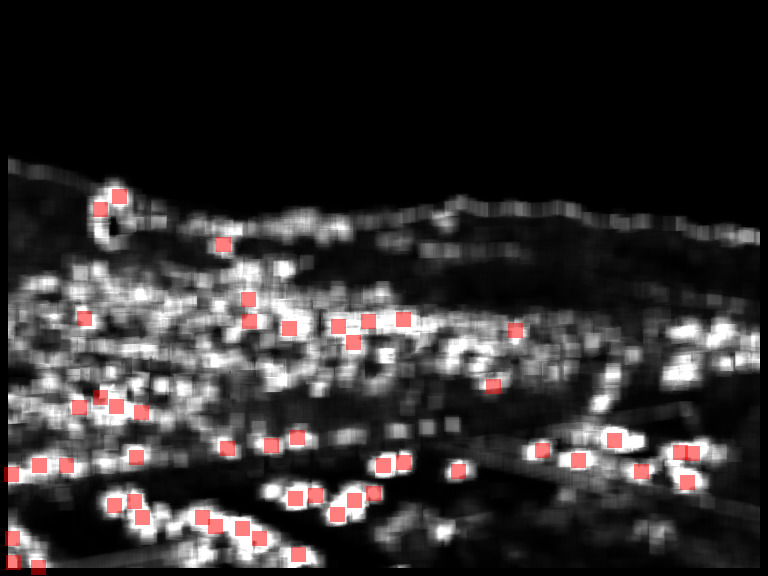
\includegraphics[scale=.3]{5-1.jpg}
  \caption{50個のとき}
  \label{5-1.jpg}
\end{figure}

\begin{figure}[ht]
  \centering
  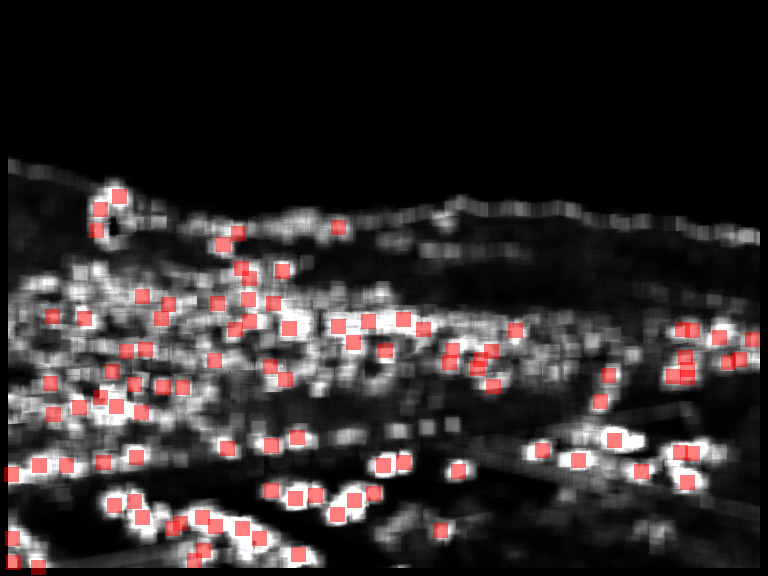
\includegraphics[scale=.3]{5-2.jpg}
  \caption{100個のとき}
  \label{5-2.jpg}
\end{figure}

\subsection{速度とメモリを効率化}
実装例で確保された領域 int kk[9999][2] の要素数は,検出され得る最大数より遥かに少なく問題が起きる可能性があると資料にあるのはうなずける.また,画素数と同数の作業領域を確保するのは無駄が多い.そこで資料を参考に,現在までに発見された点を,MAX 個まで保持できる領域を用意し,MAX+1 個目以降の追加時には,新しい候補か現在の最下位候補のどちらかを破棄することで,候補が MAX 個を越えない様にする.実装には挿入ソートを用いた.以下そのソースコードである.

\begin{verbatim}
    for(v=-W;v<=W;v++) for(u=-W;u<=W;u++){
        if(DElem(im2, x+u, y+v) > max){
          max = DElem(im2,x+u,y+v);
        }
      }
      if( max == DElem(im2, x, y) ){
        a = n;
        if(n < MAX) { n++; }
        for(;a>0 && w[a-1][2] < DElem(im2, x, y);a--){
          w[a][0]=w[a-1][0]; w[a][1]=w[a-1][1]; w[a][2]=w[a-1][2];
        }
        w[a][0]=x; w[a][1]=y; w[a][2]=max;
      }
\end{verbatim}

\section{特徴点の自動対応付け 1}
高精度のパノラマ画像を生成するには正しい射影変換行列が必要であり, このためには両方の画像で同じ物体を指している特徴点対が4組以上必要である.まず,各画像で独立に検出された特徴点群の全ての組み合わせに対して類似度を計算し,この中から同一物体を指す組を見つけ出す.最も簡単な類似度の指標は,特徴点周辺の小領域の画素値の差の2乗和(Sum of Squared Differences)である.特徴点対を選ぶ際,一つの点が複数の点と対応しないようにすることや,点の優先順位について考慮する.

\subsection{greedy.c を完成させ,第1画像の第 i 特徴点と,第2画像の第 j 特徴点の類似度(下記の値)を全てのi,jの組について計算し,行列の(i,j)要素に格納した表を作りなさい}
結果
\tiny
\begin{verbatim}
    53 124   5  59  41  55  72  53  54 116  92  63  85  35 108 101  40  61  52  83  76  56  56  53  67  69  64  57  47  92 
    66 112  38  41  59  47  56  45  54  75 102  65  84  52 100  82  50  57  51  63  70  48  50  53  56  60  55  49  44  99 
    83 120  83  83  78  77  68  43  88  63 115  78 108  74  95  46  80  56  41  61  80  49  86  62  69  50  72  79  76  99 
    43  88  51  67   9  63  61  49  32  90 101  40  66  43  92  74  44  62  45  52  54  39  42  43  54  69  61  46  35 108 
    13  96  54  69  45  85  80  59  63 121 122  52  97  54 112  96  54  68  55  68  67  56  66  63  59  91  71  58  45 103 
    76 134  32  57  49  27  50  54  48  97 115  77  95  53 119  93  59  57  62  68  83  55  58  63  64  61  64  55  56 121 
    59 117  38  42  45  40  52  49  43  81  90  57  74  43  94  70  47  51  46  61  65  41  43  40  56  57  46  42  40  94 
    82 114  55  57  65  30  34  46  58  76 103  66  90  57  91  69  63  45  44  64  69  49  55  49  61  44  46  58  56 116 
   115  98 101  81  95  75  66  47  90  21  94  79  83  90  71  26  85  41  46  71  76  63  69  58  64  29  50  60  80  89 
    78  76  68  60  64  49  38  28  57  39  86  53  56  75  61  39  62  39  43  50  54  49  46  52  53  36  34  33  47  73 
    60 119  52  58  32  47  59  46   3  90 121  63  71  46 121  76  62  60  59  53  65  45  45  63  62  70  57  41  48 129 
    62  94  55  67  60  63  51  28  67  57  51  47  59  44  48  36  47  35  15  72  59  31  54  28  52  32  33  51  52  61 
    57  54  65  55  45  78  65  52  64  70  64   4  43  51  56  68  37  53  40  57  34  49  28  36  43  54  35  32  27  62 
   124 102 102 102 111  97  76  70 135  66  41  65  68  98  14  63  75  67  51 120  83  78  74  44  70  46  47  81  80  56 
    61  93  54  58  59  44  38  39  59  67  72  44  62  45  72  44  49  11  29  57  56  41  53  35  45  33  36  37  47  85 
    56 135  36  63  51  52  61  46  51  95  80  56  75   9  91  76  46  46  32  76  70  32  61  38  55  57  48  59  55 102 
   106 100  98  90  88  85  68  47  85  46  76  70  71  92  58   3  77  41  47  81  81  63  71  49  72  38  48  51  77  72 
   138 137  94 108 121 124 111  97 140 105  22  79  69  94  44  91  74  83  60 163 111  96  77  48  95  71  67  92  92  48 
    55  88  37  61  46  61  62  47  60  96  67  36  56  39  74  77   6  54  35  76  53  50  40  32  52  62  49  45  37  65 
    65 109  56  66  49  48  50  35  53  68  83  57  82  45  67  50  62  43  27  70  67  12  59  42  44  47  44  51  53 104 
    58  63  83  69  54  68  63  46  56  72 160  61  87  78 129  79  74  58  66  10  42  62  57  80  55  64  69  50  43 129 
   103  74  89  75  75  94  80  66  81  64  66  49   6  77  61  68  61  65  59  83  58  81  48  56  71  49  39  46  55  58 
    60  50  80  52  51  78  71  56  66  73 114  36  58  61  91  81  49  64  49  38   1  56  41  61  53  62  58  41  28  89 
    62  86  57  42  62  58  53  44  76  62  74  44  69  39  52  71  45  49  28  65  41  32  47  37  33  41  38  55  40  76 
    39 116  46  62  34  55  56  43  44 102  92  42  76  31  88  75  45  50  27  65  55  30  55  38  59  62  50  50  43 113 
    54  57  52  29  48  54  63  55  48  68 101  39  55  54  91  86  43  56  56  37  29  50  26  56  31  60  50  28  16  85 
    92  88  73  69  78  59  49  35  78  31  68  58  57  65  49  35  64  28  30  64  59  51  59  43  54   5  32  52  65  65 
    59  74  64  46  48  56  44  39  53  62  78  30  49  39  58  56  44  50  32  47  29  33  38  34  45  42  26  34  31  84 
    95  63  90  63  80  87  77  54  81  33  62  55  43  84  53  34  67  52  49  65  57  64  43  48  49  37  45  44  52  42 
    70  70  58  60  48  78  71  48  55  55  63  33  39  53  70  45  40  36  40  55  52  54  32  30  52  38  36  26  39  56 
\end{verbatim}
\normalsize
表中の色の異なる要素は,次の条件を満たす様に選ばれている: (i) 各行に 1 つ,(ii) 各列に 1 つ,(iii) 色の異なる要素の合計が小さい.
第 i 行, 第 j 列に色がついているとき,第1画像の第 i 特徴点と第2画像の第 j 特徴点が同一の物体であると期待される.

\subsection{上記の条件(i)–(iii)の意味を考察しなさい.}
(i)(ii) 画像1に対して画像2の特徴点が複数選ばれないことを意味している.
(iii) 画像1と画像2の特徴点の類似度が高いということを意味している

\subsection{方法1の問題点}
\begin{itemize}
    \item SSDの和が方法2と比べて大きいので精度がよくない.
    \item もし対応する特徴点が二枚目の画像にないときはすごく異なる対応点が選ばれてしまう.
    \item 同じ列に選ばれた点よりもとても強い特徴点がいても選ばれないことがある.
  \end{itemize}

\subsection{方法2の問題点}
\begin{itemize}
    \item 方法1同様,もし対応する特徴点が二枚目の画像にないときはすごく異なる対応点が選ばれてしまう.
    \item INFINITYで上書きしたものは本当にいらないものなのかどうかの判断ができていない.
  \end{itemize}

\subsection{実装例1をgreedy.cに追加し,動作させなさい.また,これをもとに方法2を完成させなさい}
以下が方法2のソースコードである.点の数だけ対応を見つける際に,各行,各列の最小値を見つけて,かぶらないようにその点の横と縦を見ないようにする動作をしている.
\begin{verbatim}
    int matchMethod2(double w[][4],Matrix*mt,Image*im ,
    int x1[][2],int N1,Image*im2,int x2[][2],int N2){
  int i,j,k,l,n = 0;
  int minElem[3] = {0,0,INFINITY_INT};
  // SSDの表中の最小値
  for(i=0;i<MAX;i++){//点の数
    for(j=0;j<mt->W;j++){//横幅
      for(k=0;k<mt->H;k++){//縦幅
        if(Elem(mt,j,k) < minElem[2]){
          minElem[0] = j;
          minElem[1] = k;
          minElem[2] = (int)Elem(mt,j,k);
          //printf("%d,%d,%d\n",minElem[0],minElem[1],minElem[2]);
        }
      }
    }
    for(k=0;k<MAX;k++) Elem(mt,minElem[0],k)=INFINITY_INT;//横固定
    for(k=0;k<MAX;k++) Elem(mt,k,minElem[1])=INFINITY_INT;//縦固定
    //MatrixPrint(mt);
    printf("%d,%d,%d,%d,\n",x1[minElem[0]][0],x1[minElem[0]][1],
    x2[minElem[1]][0],x2[minElem[1]][1]);
    w[n][0] = x1[minElem[0]][0];
    w[n][1] = x1[minElem[0]][1];
    w[n][2] = x2[minElem[1]][0];
    w[n][3] = x2[minElem[1]][1];
    n++;
    minElem[2]=INFINITY_INT;
  }
  return n;
}
\end{verbatim}
\subsection{4組の特徴点対を選び,射影変換行列を計算し,合成画像を作成しなさい.}
算出した特徴点
\begin{verbatim}
    315,495,564,507,
    259,538,507,548,
    119,196,367,211,
    142,517,393,522,
\end{verbatim}

出力した画像は図\ref{6-1.jpg}に記載した.

\begin{figure}[ht]
    \centering
    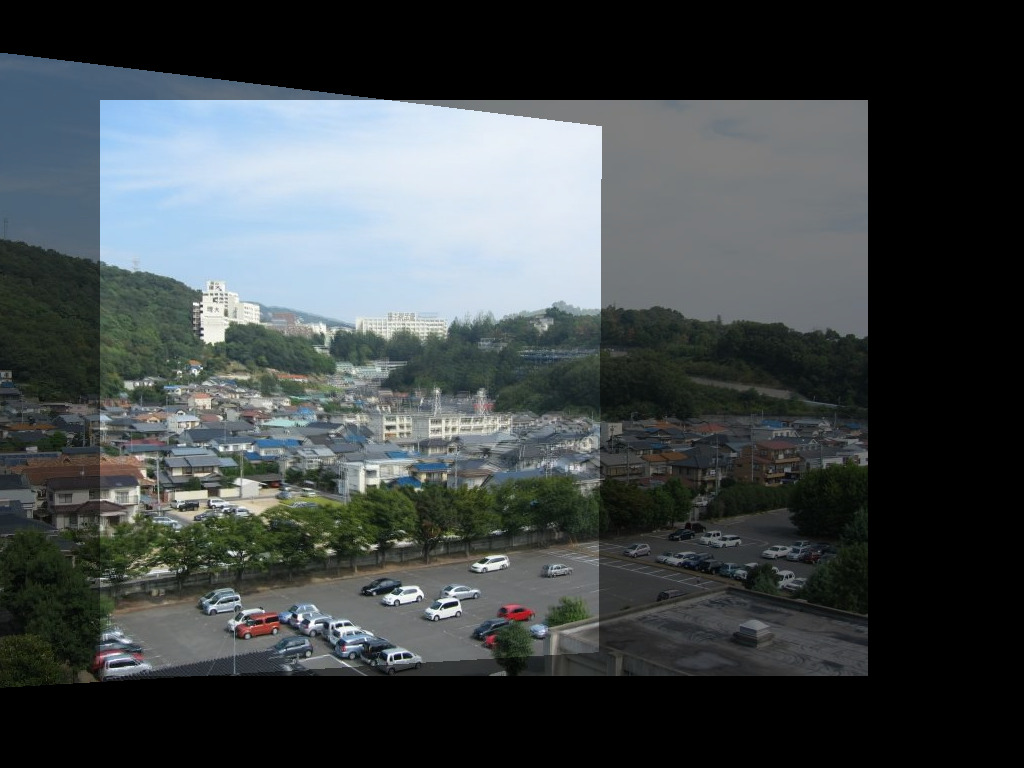
\includegraphics[scale=.3]{6-1.jpg}
    \caption{結果}
    \label{6-1.jpg}
\end{figure}

\subsection{下記の観点で考察または実装しなさい.}
SSD(i,j) の表の作成は,N1やN2が大きい時にはかなりの演算を要する.
\subsubsection{calcSSDtable の i のループをopenMPで並列化することは容易である.}

実際に,これはループの前に\verb|#pragma omp parallel for private (j)|の記載をつけ,fopenmpオプションをつけてコンパイルし,実行できた

\section{特徴点の自動対応付け 2}
厳密解法や全解探索が難しい問題でも,乱数によって近似的に扱える場合がある.ここでは RANSAC と呼ばれるアルゴリズムを用いて特徴点の自動対応付けを行う.

\subsection{RANSAC(あるいは独自の方法)で自動対応付けを実現し,画像を合成しなさい}

パノラマ画像での各画像から抽出してきた特徴量は,もう一方の画像に対応点が存在していない「外れ値」が含まれており,最小二乗法によりどの点とどの点が対応するかを計算すると,外れ値ではうまく対応関係が作れない.そこで、パノラマ画像作成での対応点計算にはRANSACにより外れ値は見ないような上手い対応点を見つける.

RANSACでは以下の3つの手続きを最適な評価値(スコア)が(3)で出てくるまで繰り返す


(1):あらかじめ決めておいたサンプル数nだけランダムにデータをサンプリング


(2):サンプルしたn個のデータを用い,モデルのパラメータを算出(最小二乗法で誤差を最小化)


(3):処理2で求めたモデルのパラメータに対して、あらかじめ範囲を決めておいた閾値内のデータのみを用いて,どれくらい正しいかのスコアを評価

この(1)~(3)の処理による各繰り返しにおいて,外れ値ではない正しい特徴点ができているかを判断する.

\subsubsection{問題点}
試行回数が少ないと上手く合成できない.閾値が適正でないと上手く合成できない.

\subsubsection{改善策}
試行回数を増やし,閾値を小さくすることで改善できた.
試行回数は対応点集合の中に含まれる誤りの割合を p とすることで見積もることができるが今回は余力がないためやっていない.

\subsection{合成結果が芳しくない場合は,w[]に用意する候補数,「重なり」,試行回数等を変える.}

実験結果の図\ref{7-1.jpg}は閾値を5,試行回数を100万回にして行った.

閾値が大きいと上手く出ず,試行回数が少なくても上手く出なかった.

\subsection{下記の観点で考察または実装しなさい}
\subsubsection{4つの乱数(i0,i1,i2,i3)を発生させるとき,同じものが2度以上選ばれないようにする方法}
以下実装したソースコードである.
\begin{verbatim}
    void initRndAry(int rndAry[MAX]){
        for(int i = 0; i<MAX; i++){
            rndAry[i] = i;
        }
        srand(__rdtsc()); // __rdtsc については第4回を参照
    }

    void chooseFourNumbers(int rndAry[MAX]){
        for(int i=0;i<4;i++){
            int j, t;
            j = (int)((long long)rand()*(MAX-i)/(RAND_MAX+1LL))+i; // 乱数関数は stdlib.h で宣言されている.
            t = rndAry[i]; 
            rndAry[i] = rndAry[j]; 
            rndAry[j] = t;
        }
    }
\end{verbatim}
rndAry は,0 から MAX-1 までの数を 1 つずつ保持している. この配列の内容を入れ替える操作によって,数値の順序は変わるが,
全ての数値が一回づつ現れる性質は変わらないため, 相異なる数個の乱数が得られる.

上記の rndAry[0] から rndAry[3] を使う部分では,配列 w[][4] から4行を選んで変換行列を算出する
以下にそのソースコードを示した.

\begin{verbatim}
    void calcHomography(double H[3][3],double w[][4],int rndAry[MAX], 
    Matrix *cmA, Matrix *vt, Matrix *mtR, Matrix *tmp){
    int a = rndAry[0], b = rndAry[1], c = rndAry[2], d = rndAry[3];
    double ww[][4] = {
        w[a][0], w[a][1], w[a][2], w[a][3],
        w[b][0], w[b][1], w[b][2], w[b][3],
        w[c][0], w[c][1], w[c][2], w[c][3],
        w[d][0], w[d][1], w[d][2], w[d][3],
    };
      // create A (col-major)
    for(int i=0;i<4;i++){
        Elem(cmA,0,i*2  )=ww[i][0];
        Elem(cmA,1,i*2  )=ww[i][1];
        Elem(cmA,2,i*2  )=1;
        Elem(cmA,3,i*2  )=0;
        Elem(cmA,4,i*2  )=0;
        Elem(cmA,5,i*2  )=0;
        Elem(cmA,6,i*2  )=-ww[i][0]*ww[i][2];
        Elem(cmA,7,i*2  )=-ww[i][1]*ww[i][2];
        Elem(cmA,0,i*2+1)=0;
        Elem(cmA,1,i*2+1)=0;
        Elem(cmA,2,i*2+1)=0;
        Elem(cmA,3,i*2+1)=ww[i][0];
        Elem(cmA,4,i*2+1)=ww[i][1];
        Elem(cmA,5,i*2+1)=1;
        Elem(cmA,6,i*2+1)=-ww[i][0]*ww[i][3];
        Elem(cmA,7,i*2+1)=-ww[i][1]*ww[i][3];
        Elem(vt ,0,i*2  )=ww[i][2];
        Elem(vt ,0,i*2+1)=ww[i][3];
    }
    MatrixQRDecompColMajor(mtR,cmA);
    MatrixMultT(tmp,vt,cmA);
    MatrixSimeqLr(tmp,mtR);

    H[0][0] = Elem(tmp,0,0);
    H[0][1] = Elem(tmp,0,1);
    H[0][2] = Elem(tmp,0,2);
    H[1][0] = Elem(tmp,0,3);
    H[1][1] = Elem(tmp,0,4);
    H[1][2] = Elem(tmp,0,5);
    H[2][0] = Elem(tmp,0,6);
    H[2][1] = Elem(tmp,0,7);
    H[2][2] = 1;
}
\end{verbatim}

そして,変換行列の信頼度を評価するため,上記の「検出された点と変換された点の距離が十分に小さい点」の数を計算する.
以下そのソースコード部分である.
\begin{verbatim}
    int calcScore(double H[3][3], double w[][4]){
        int score=0;
        for(int i=0;i<MAX;i++){
            double x=w[i][0], y=w[i][1], u=w[i][2], v=w[i][3],
            x_prime = H[0][0] * x + H[0][1] * y + H[0][2],
            y_prime = H[1][0] * x + H[1][1] * y + H[1][2],
            z_prime = H[2][0] * x + H[2][1] * y + H[2][2], // 変換行列と (x,y,1)^T の積
            du = (x_prime/z_prime) - u,
            dv = (y_prime/z_prime) -v; // (x,y) を変換した座標(第2回の概要を参照)と (u,v) の差
            if(du*du+dv*dv < 10) score++;//w[i] は正しい;
            else score += 0;              //w[i] は正しくない;
        }
        return score;
    }    
\end{verbatim}

この実装により得られた画像は図\ref{7-1.jpg}に示した.

\begin{figure}[ht]
    \centering
    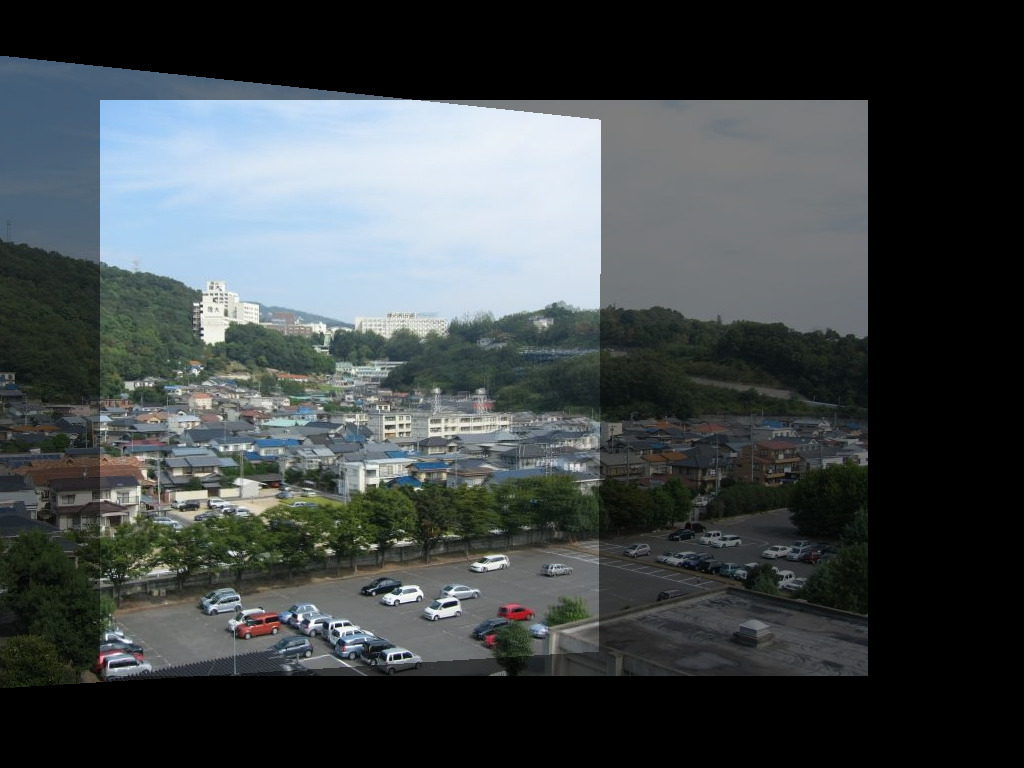
\includegraphics[scale=.5]{7-1.jpg}
    \caption{結果}
    \label{7-1.jpg}
\end{figure}

\section{まとめ}
これまでの内容をまとめて,入力された2枚以上の画像を自動で合成するプログラムを作成した.ここではその問題点と工夫した点について述べる.


実装したソースコードは第\ref{sec:code}章にまとめて記述する.内容は出力画像領域を確保し,第1画像を読み込む.画像から特徴点を検出し,有効な点を選び出す.第2画像を読み込む.画像から特徴点を検出し,有効な点を選び出す.貪欲法・RANSAC等を用い適切な4組の対応点を選び,変換行列を算出する.前項で得られた変換行列をほぼ満たすn組の対応点を使って,より良い変換行列を算出する.第1画像と第2画像を合成.その後,第3画像を読み込み,同様の処理を行い,第2画像と合成した後,すべての3枚を張り合わせたものを画像ファイルに出力するという動作である.

\subsection{問題点}
今回作成したパノラマ画像のプログラムは,3枚の入力しか対応しておらず,入力された画像の枚数に応じて動的に画像を描画してくれるものではない.


また,一部並列動作や分解などを行っていないため,高速なプログラムにはなっていないこと.


合成する他方の画像に対応する特徴点が見つけられない場合に上手く画像を合成できないこと.

異なる視点からの画像だと合成がうまくできないこと.

\subsection{工夫した点}
2枚でなく,3枚で合成ができるようにした.


画像によって上手く特徴点を見つけられる閾値が違うので,コマンドラインで実行をするときに閾値と,走査する範囲を指定できるようにした.第2から第4引数までが画像のデータで,第4引数が閾値,第5引数が15x15などの走査範囲の指定である.
\begin{verbatim}
    実行例
    ./a.out IMAG1537.jpg IMAG1538.jpg IMAG1539.jpg 4 5
\end{verbatim}

MatrixLocalMaxという特徴点がいいものか見る関数の処理量が大きいため,縦の走査と横の走査で処理を分解し,なるべく軽い動作にしたこと.

自分の画像で合成結果を試したこと.撮る画像によっては上手く特徴点を見つけられないことがあり,そもそも画像の撮り方に苦戦をした.

image.cという1つのファイルにまとめることで,image.hをヘッダーに読み込むようにして,コンパイル時の指定を少なくし,構造的にも1つのファイルに複数の関数が並ばないように役割を決めた作成にした.

\subsection{自分で撮影した写真の合成を試みなさい}

作成したプログラムを用いて撮影した画像を合成することを試みた.当初,黒いキーボードの上に,白い色のマスコットを置いた画像で行っていた.しかし,いくら閾値などを変えても特徴点を4点も見つけられなかったり,best\_scoreの値が4とか6であまり大きな値を見つけられず失敗した.図\ref{8-1.jpg}がその結果である
\begin{figure}[ht]
    \centering
    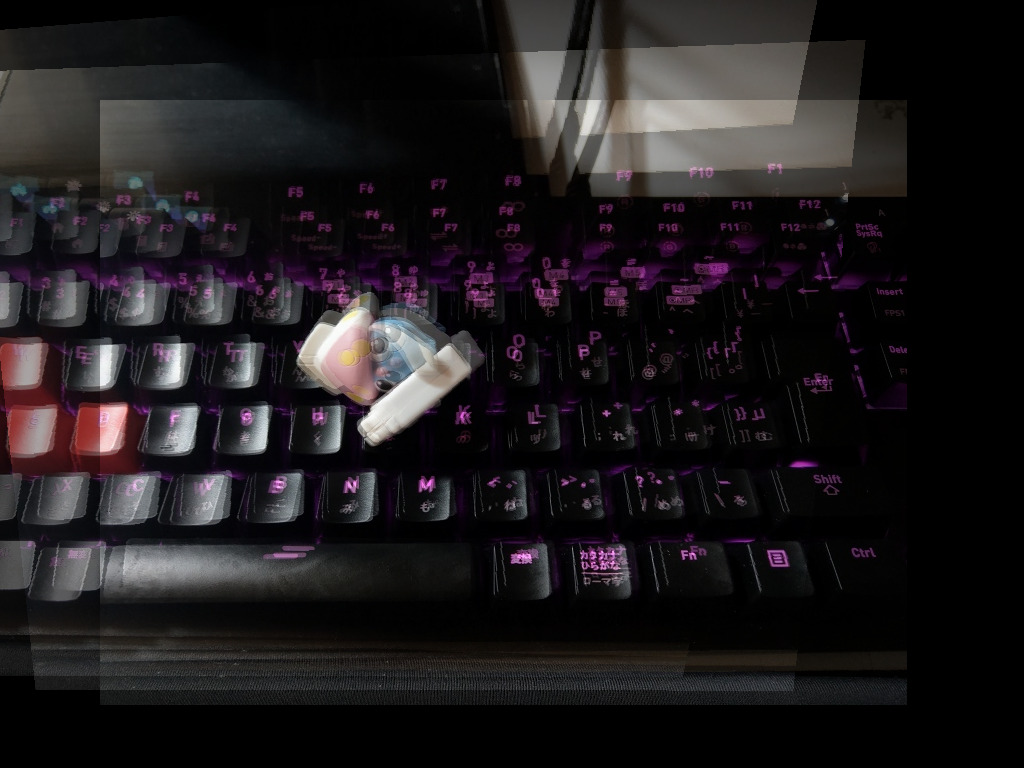
\includegraphics[scale=.5]{8-1.jpg}
    \caption{自分での合成結果1}
    \label{8-1.jpg}
\end{figure}

その後,どうにか特徴点らしきものが多く出そうな画像を撮って行い閾値や走査する範囲を変えてみると先程よりは上手く合成できた.図\ref{8-2.jpg}がその結果である.
\begin{figure}[ht]
    \centering
    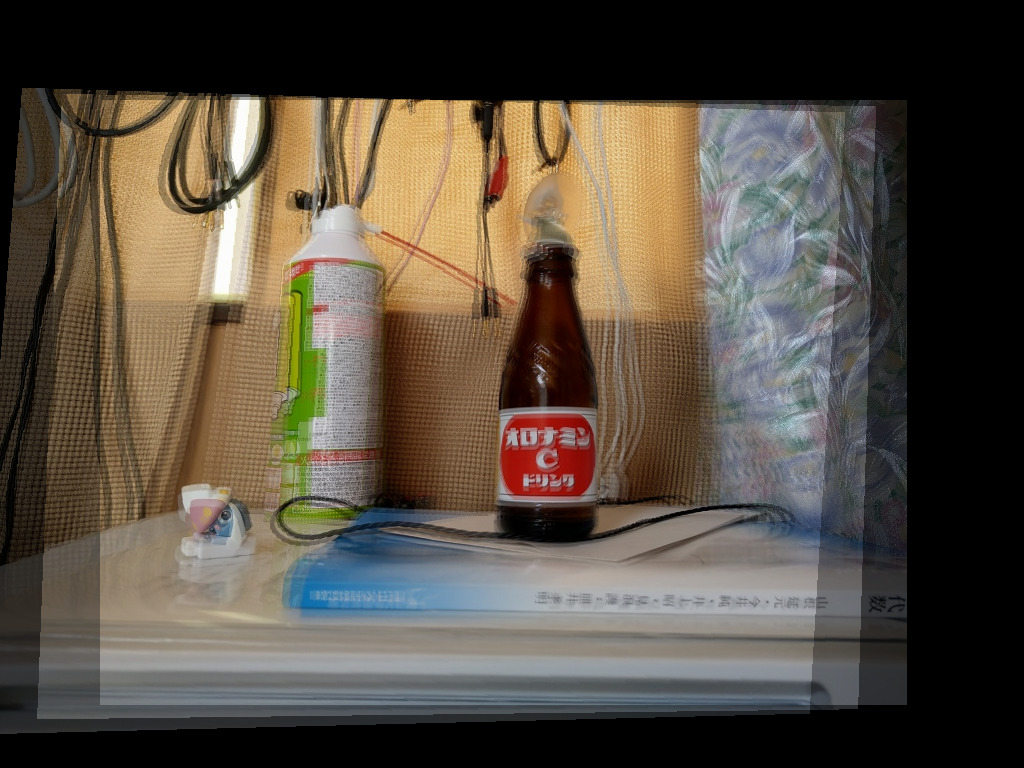
\includegraphics[scale=.5]{8-2.jpg}
    \caption{自分での合成結果2}
    \label{8-2.jpg}
\end{figure}



\section{感想}
本講義では,複数枚のパノラマ画像の合成についての基本的な内容についての実際の実装方法を実装することで,その内部処理および画像処理の仕組みの一部について知ることができたように思う.GPUによる実装や,妥当な行列が得られるまでの試行回数の見積もり,遥かにより効率的な特徴点数が多い時の類似度の表から最小値をk回捜し出すcalcSSDtable関数の実装などの米印2つの発展課題などに取り組む余力がなかったが,今回の実験で画像処理について興味が湧いたので取り組んでみたい.

\section{実装したコード}
\label{sec:code}

\tiny

\subsection{image.h}

\begin{verbatim}
    #pragma once

#include<stdio.h>
#include<stdlib.h>
#include<math.h>
#include<string.h>

typedef struct _Image
{
    unsigned char *data;
    int W, H;
} Image;

typedef struct {
  double *data;
  int W,H;
} Matrix;

#define IElem(_im, _x, _y, _c) (_im)->data[(_y) * (_im)->W * 3 + (_x)*3 + (_c)]
#define Elem(_a,_b,_c)  (_a)->data[(_a)->W*(_b)+(_c)]
#define DElem(_a,_b,_c)  (_a)->data[(_a)->W*(_c)+(_b)]
#define Row(_a,_b)     ((_a)->data+(_a)->W*(_b))
#define isInsideImage(is, u, v) (0 <= u && u < is->W && 0 <= v && v < is->H)
#define MAX 30

#ifdef _WIN32
#include<intrin.h>
#else
#define __rdtsc() ({ long long a,d; __asm__ volatile ("rdtsc":"=a"(a),"=d"(d)); d<<32|a; })
#endif

Image *ImageAlloc(int W, int H);
Image *ImageRead(const char *name);
void ImageFree(Image *im);
void ImageWrite(const char *name, Image *im);
void ImageClear(Image *im);
void ImageImageProjectionAlpha(Image *id, Image *is, double a[3][3], double alpha);
void ImageDrawBox(Image *im, int x, int y,int W);
void mult33(double d[3][3],double a[3][3],double b[3][3]);
Matrix *MatrixAlloc(int _H,int _W);
double ImageSSD(Image*im,int x1,int y1, Image*im2,int x2,int y2,int W);
void calcSSDtable(Matrix*mt,Image*im ,int x1[][3],int N1,Image*im2,int x2[][3],int N2, int W);
int matchMethod1(double w[][4],Matrix*mt,Image*im ,int x1[][3],int N1,Image*im2,int x2[][3],int N2);
int matchMethod2(double w[][4],Matrix*mt,Image*im ,int x1[][3],int N1,Image*im2,int x2[][3],int N2);
void ImageFeature(Matrix*im2,Image*im,int W);
int MatrixLocalMax(int w[][3], Matrix*im2, int W);
void MatrixSimeqLr(Matrix*mtB,Matrix*mtR);
void MatrixQRDecompColMajor(Matrix*mtR,Matrix*mt);
void MatrixCopyT(Matrix*mtD,Matrix*mt);
void MatrixClear(Matrix*mt);
void MatrixCopy(Matrix*mtD,Matrix*mt);
void VSA(double*d,double*a,double s,int N);
void VSS(double*d,double s,int N);
double VP(double*a,double*b,int N);
\end{verbatim}

\subsection{image.c}
\begin{verbatim}
#include "image.h"

union {int i; float f;} _inf={0x7f800000};
#define INFINITY _inf.f // 2重定義エラーが出るなら,この定義を削除
#define INFINITY_INT _inf.i

Image *ImageAlloc(int w, int h)
{
    Image *im = (Image *)malloc(sizeof(Image));
    im->W = w;
    im->H = h;
    im->data = (unsigned char *)malloc(3 * w * h);
    return im;
}

void ImageClear(Image *im){
    for(int y=0;y<im->H;y++){
        for(int x=0;x<im->W;x++){
            IElem(im,x,y,0) = 0;
            IElem(im,x,y,1) = 0;
            IElem(im,x,y,2) = 0;
        }
    }
}
void mult33(double d[3][3],double a[3][3],double b[3][3]){
    for(int i=0;i<3;i++){
        for(int j=0;j<3;j++){
            d[i][j] = a[i][0]*b[0][j] + a[i][1]*b[1][j] + a[i][2]*b[2][j];
        }
    }
}

void ImageImageProjectionAlpha(Image*id,Image*is,double a[3][3],double alpha){
  int x,y,u,v;
  double r;
  for(y=0;y<id->H;y++) for(x=0;x<id->W;x++){
    r=1/(a[2][0]*x+a[2][1]*y+a[2][2]);
    u=r*(a[0][0]*x+a[0][1]*y+a[0][2]);
    v=r*(a[1][0]*x+a[1][1]*y+a[1][2]);
    if( isInsideImage(is,u,v) ){
      IElem(id,x,y,0)+=IElem(is,u,v,0)*alpha,
      IElem(id,x,y,1)+=IElem(is,u,v,1)*alpha,
      IElem(id,x,y,2)+=IElem(is,u,v,2)*alpha;
    }
  }
}

Matrix *MatrixAlloc(int _H,int _W){
  Matrix*mt=(Matrix*)malloc(sizeof(Matrix));
  mt->W = _W;
  mt->H = _H;
  mt->data=(double*)malloc(mt->W*mt->H*sizeof(double));
  return mt;
}

Image *ImageRead(const char *name)
{
    int W, H;
    Image *im;
    char tmp[128];
    sprintf(tmp, "convert %s ppm:-", name);
    FILE *fp = popen(tmp, "r");
    if (fp == NULL)
    {
        fprintf(stderr, "could not read %s\n", name);
        return 0;
    }
    fscanf(fp, "%*s%d%d%*s%*c", &W, &H);
    //fprintf(stderr,"w x h=%d %d\n",W,H);
    im = ImageAlloc(W, H);
    fread(im->data, 1, W * H * 3, fp);
    pclose(fp);
    return im;
}

void ImageWrite(const char *name, Image *im)
{
    char tmp[128];
    sprintf(tmp, "convert ppm:- %s", name);
    FILE *fp = popen(tmp, "w");
    if (fp == NULL)
    {
        fprintf(stderr, "could not write %s\n", name);
        return;
    }
    fprintf(fp, "P6 %d %d 255\n", im->W, im->H);
    fwrite(im->data, 1, im->W * im->H * 3, fp);
    pclose(fp);
}

double ImageSSD(Image*im,int x1,int y1, Image*im2,int x2,int y2,int W){
  int i,j;
  double sr=0,sg=0,sb=0,dr,dg,db;
  for(i=-W;i<=W;i++) for(j=-W;j<=W;j++){
    dr  = IElem(im, x1+j, y1+i, 0) - IElem(im2, x2+j , y2+i, 0);
    dg  = IElem(im, x1+j, y1+i, 1) - IElem(im2, x2+j , y2+i, 1);
    db  = IElem(im, x1+j, y1+i, 2) - IElem(im2, x2+j , y2+i, 2);
    sr += dr*dr;
    sg += dg*dg;
    sb += db*db;
  }
  return sr+sg+sb;
}

void calcSSDtable(Matrix*mt,Image*im ,int x1[][3],int N1,Image*im2,int x2[][3],int N2,int W){
    int i,j;
    #pragma omp parallel for private (j)
    for(i=0;i<N1;i++){
        for(j=0;j<N2;j++){
            Elem(mt,i,j) = ImageSSD(im ,x1[i][0],x1[i][1],im2,x2[j][0],x2[j][1], W);
        }
    }
}

int matchMethod1(double w[][4],Matrix*mt,Image*im ,int x1[][3],int N1,Image*im2,int x2[][3],int N2){
  int i,j,k,ji,n=0;

  for(i=0;i<N1;i++){
    double sm=INFINITY,t;
    for(j=0;j<N2;j++){
      t = Elem(mt,i,j);
      if(sm>t) sm=t, ji=j;
    }
    //printf("%d,%d,%d,%d,\n",x1[i][0],x1[i][1],x2[ji][0],x2[ji][1]);
    // 上の printf で表示されるものを w[n][] に格納.
    w[n][0] = x1[i][0];
    w[n][1] = x1[i][1];
    w[n][2] = x2[ji][0];
    w[n][3] = x2[ji][1];
    n++;
    for(k=0;k<N1;k++) { Elem(mt,k,ji)=INFINITY; }
  }
  printf("%d\n",n);
  return n;
}

int matchMethod2(double w[][4],Matrix*mt,Image*im ,int x1[][3],int N1,Image*im2,int x2[][3],int N2){
  int i,j,k,l,n = 0;
  int minElem[3] = {0,0,INFINITY_INT};
  // SSDの表中の最小値
  for(i=0;i<MAX;i++){//点の数だけ
    for(j=0;j<mt->W;j++){//横幅
      for(k=0;k<mt->H;k++){//縦幅
        if(Elem(mt,j,k) < minElem[2]){
          minElem[0] = j;
          minElem[1] = k;
          minElem[2] = (int)Elem(mt,j,k);
          //printf("%d,%d,%d\n",minElem[0],minElem[1],minElem[2]);
        }
      }
    }
    for(k=0;k<MAX;k++) Elem(mt,minElem[0],k)=INFINITY_INT;//横固定して爆破
    for(k=0;k<MAX;k++) Elem(mt,k,minElem[1])=INFINITY_INT;//縦固定して爆破
    //MatrixPrint(mt);
    //printf("%d,%d,%d,%d,\n",x1[minElem[0]][0],x1[minElem[0]][1],x2[minElem[1]][0],x2[minElem[1]][1]);
    w[n][0] = x1[minElem[0]][0];
    w[n][1] = x1[minElem[0]][1];
    w[n][2] = x2[minElem[1]][0];
    w[n][3] = x2[minElem[1]][1];
    n++;
    minElem[2]=INFINITY_INT;
  }
  return n;
}

void ImageFeature(Matrix*im2,Image*im,int W){//特徴点らしさ
  int x,y,u,v,ix,iy;
  for(y=W+1;y<im->H-W-1;y++) for(x=W+1;x<im->W-W-1;x++){
        double ixx,ixy,iyy;
        ixx=iyy=ixy=0;
        for(v=-W;v<=W;v++)for(u=-W;u<=W;u++){
            ix = IElem(im, x+u+1, y+v, 1) - IElem(im, x+u-1, y+v, 1);
            iy = IElem(im, x+u, y+v+1, 1) - IElem(im, x+u, y+v-1, 1);
            ixx += ix*ix; // ixx だけでなく ixy,iyy も計算する. 
            iyy += iy*iy;
            ixy += ix*iy;
    }
    DElem(im2,x,y) = ((ixx + iyy)-sqrt(pow(ixx+iyy,2.0)-4.0*(ixx*iyy-ixy*ixy)))/2.0; 
  }
}

int MatrixLocalMax(int w[][3], Matrix*im2, int W){//特徴点がほんとにそうかどうか
  int x,y,u,v,n=0,a;
  for(y=W+1;y<im2->H-W-1;y++) for(x=W+1;x<im2->W-W-1;x++){
    double max=-1;
    for(v=-W;v<=W;v++) for(u=-W;u<=W;u++){
      if(DElem(im2, x+u, y+v) > max){
        max = DElem(im2,x+u,y+v);
      }
    }
    if( max == DElem(im2, x, y) ){
      a = n;
      if(n < MAX) { n++; }
      for(;a>0 && w[a-1][2] < DElem(im2, x, y);a--){
        w[a][0]=w[a-1][0]; w[a][1]=w[a-1][1]; w[a][2]=w[a-1][2];
      }
      w[a][0]=x; w[a][1]=y; w[a][2]=max;
    }
  }
  return n; // 記録した点の数 
}
double VP(double*a,double*b,int N){
  double s=0;
  int i;
  for(i=0;i<N;i++) s += a[i] * b[i] ;
  return s;
}
void VSS(double*d,double s,int N){
  int i;
  for(i=0;i<N;i++) d[i] *= s;
}

void VSA(double*d,double*a,double s,int N){
  int i;
  for(i=0;i<N;i++) d[i] += a[i] * s;
}
void MatrixClear(Matrix*mt){
  memset(mt->data,0,mt->W*mt->H*sizeof(double));
}


void MatrixCopy(Matrix*mtD,Matrix*mt){
  memmove(mtD->data,mt->data,mt->W*mt->H*sizeof(double));
}

void MatrixCopyT(Matrix*mtD,Matrix*mt){
  int i,j;
  for(i=0;i<mtD->H;i++)
    for(j=0;j<mtD->W;j++)
      Elem(mtD,i,j) = Elem(mt,j,i);
}
void MatrixMultT(Matrix*mtD,Matrix*mtA,Matrix*mtB){
  // D = A B^T
  int i,j;
  for(i=0;i<mtA->H;i++){
      for(j=0;j<mtB->H;j++){
        Elem(mtD,i,j) = VP( Row(mtA,i), Row(mtB,j), mtA->W);
    }
  }
}
void MatrixQRDecompColMajor(Matrix*mtR,Matrix*mt){
  double t;
  int W = mt->W;
  double **aT = (double **)malloc((sizeof (double *)) * mt->H);
  for(int get=0; get<mt->H;get++){
    aT[get] = Row(mt,get);
  }
  MatrixClear(mtR);
  for(int i=0; i < W; i++){
    for(int j=0; j <= i; j++){
      if(j == i){
        Elem(mtR,j,i) = t = sqrt(VP(aT[j],aT[i],W));
        VSS(aT[i], 1/t, W);
      }else{
        Elem(mtR,j,i) = t = VP(aT[j], aT[i], W);
        VSA(aT[i], aT[j], -t, W);
      }
    }
  }
}

void MatrixSimeqLr(Matrix*mtB,Matrix*mtR){
  // B = B L^{-1}
  double * B = Row(mtB,0);
  for(int i=mtR->W-1; 0<=i; i--){
    for(int j=i+1; j<mtR->W; j++){
      B[i] -=  B[j]*Elem(mtR,i,j);
    }
    B[i] = B[i] / Elem(mtR,i,i);
  }
}
\end{verbatim}

\subsection{all.c}
\begin{verbatim}
    #include "image.h"

#define TRIAL 1000000

void initRndAry(int rndAry[MAX]){
    for(int i = 0; i<MAX; i++){
        rndAry[i] = i;
    }
    srand(__rdtsc()); // __rdtsc については第4回を参照.
}

void chooseFourNumbers(int rndAry[MAX]){
    for(int i=0;i<4;i++){
        int j, t;
        j = (int)((long long)rand()*(MAX-i)/(RAND_MAX+1LL))+i; // 乱数関数は stdlib.h で宣言されている.
        t = rndAry[i]; 
        rndAry[i] = rndAry[j]; 
        rndAry[j] = t;
    }
}

void calcHomography(double H[3][3],double w[][4],int rndAry[MAX], Matrix *cmA, Matrix *vt, Matrix *mtR, Matrix *tmp){
    int a = rndAry[0], b = rndAry[1], c = rndAry[2], d = rndAry[3];
    double ww[][4] = {
        w[a][0], w[a][1], w[a][2], w[a][3],
        w[b][0], w[b][1], w[b][2], w[b][3],
        w[c][0], w[c][1], w[c][2], w[c][3],
        w[d][0], w[d][1], w[d][2], w[d][3],
    };
      // create A (col-major)
    for(int i=0;i<4;i++){
        Elem(cmA,0,i*2  )=ww[i][0];
        Elem(cmA,1,i*2  )=ww[i][1];
        Elem(cmA,2,i*2  )=1;
        Elem(cmA,3,i*2  )=0;
        Elem(cmA,4,i*2  )=0;
        Elem(cmA,5,i*2  )=0;
        Elem(cmA,6,i*2  )=-ww[i][0]*ww[i][2];
        Elem(cmA,7,i*2  )=-ww[i][1]*ww[i][2];
        Elem(cmA,0,i*2+1)=0;
        Elem(cmA,1,i*2+1)=0;
        Elem(cmA,2,i*2+1)=0;
        Elem(cmA,3,i*2+1)=ww[i][0];
        Elem(cmA,4,i*2+1)=ww[i][1];
        Elem(cmA,5,i*2+1)=1;
        Elem(cmA,6,i*2+1)=-ww[i][0]*ww[i][3];
        Elem(cmA,7,i*2+1)=-ww[i][1]*ww[i][3];
        Elem(vt ,0,i*2  )=ww[i][2];
        Elem(vt ,0,i*2+1)=ww[i][3];
    }
    MatrixQRDecompColMajor(mtR,cmA);
    MatrixMultT(tmp,vt,cmA);
    MatrixSimeqLr(tmp,mtR);

    H[0][0] = Elem(tmp,0,0);
    H[0][1] = Elem(tmp,0,1);
    H[0][2] = Elem(tmp,0,2);
    H[1][0] = Elem(tmp,0,3);
    H[1][1] = Elem(tmp,0,4);
    H[1][2] = Elem(tmp,0,5);
    H[2][0] = Elem(tmp,0,6);
    H[2][1] = Elem(tmp,0,7);
    H[2][2] = 1;
}

int calcScore(double H[3][3], double w[][4], int limit){
    int score=0;
    for(int i=0;i<MAX;i++){
        double x=w[i][0], y=w[i][1], u=w[i][2], v=w[i][3],
        x_prime = H[0][0] * x + H[0][1] * y + H[0][2],
        y_prime = H[1][0] * x + H[1][1] * y + H[1][2],
        z_prime = H[2][0] * x + H[2][1] * y + H[2][2], // 変換行列と (x,y,1)^T の積
	    du = (x_prime/z_prime) - u,
        dv = (y_prime/z_prime) -v; // (x,y) を変換した座標(第2回の概要を参照)と (u,v) の差
        if(du*du+dv*dv <= limit) score++;//w[i] は正しい;
        else score += 0;              //w[i] は正しくない;
    }
    return score;
}

// void createPanorama(Matrix *id, Image *im, Image *im2, int bestH[3][3]){
//     double m0d[3][3]={
//       1,0,-100,
//       0,1,-100,
//       0,0,1
//     },m1d[3][3];
//     ImageImageProjectionAlpha(id,im,m0d,.5);
//     mult33(m1d,bestH,m0d);
//     ImageImageProjectionAlpha(id,im2,m1d,.5);
//     ImageWrite("panorama.jpg",id);
// }

int main(int ac,char**av){
    Image *im, *im2, *im3;
    Matrix *imf, *mt, *id;
    int N1, N2, N3, nm;
    double w[999][4];
    int x1[MAX+1][3], x2[MAX+1][3], x3[MAX+1][3];

    double m0d[3][3]={
      1,0,-100,
      0,1,-100,
      0,0,1
    },m1d[3][3],m2d[3][3];

    // 多数の変換行列から最も信頼度の高い行列を選ぶ(RANSAC)
    double bestH[3][3]; 
    int best_score = 0; // 既に発見された最良の変換行列と得点
    int rndAry[MAX];
    Matrix *cmA, *vt, *mtR, *tmp; // 作業領域をここで確保して calcHomography で使う

    /*av[1] = Wの値,それ以降は画像ファイル名*/
    im = ImageRead(av[1]);
    printf("read1\n");

    im2 = ImageRead(av[2]);
    printf("read2\n");

    imf = MatrixAlloc(im->H, im->W);

    ImageFeature(imf, im, atoi(av[5]));
    N1 = MatrixLocalMax(x1, imf, atoi(av[5]));
    printf("N1:%d\n",N1);

    ImageFeature(imf, im2, atoi(av[5]));
    N2 = MatrixLocalMax(x2, imf, atoi(av[5]));
    printf("N2:%d\n",N2);

    mt = MatrixAlloc(N1, N2);
    printf("mt\n");

    calcSSDtable(mt, im, x1, N1, im2, x2, N2, atoi(av[5]));
    printf("calcSSDtable\n");

    nm = matchMethod2(w, mt, im, x1, N1, im2, x2, N2);
    printf("nm:%d\n",nm);

    // 多数の変換行列から最も信頼度の高い行列を選ぶ(RANSAC)
    cmA = MatrixAlloc(8,8);
    vt = MatrixAlloc(1,8);
    mtR = MatrixAlloc(8,8);
    tmp = MatrixAlloc(1,8);
    printf("Alloc:cmA,vt,mtR,tmp\n");

    initRndAry(rndAry);
    printf("init andary\n");

    for(int trial = 0; trial<TRIAL; trial++){

        double H[3][3]; // 選んだ4点から計算される変換行列の置き場
        chooseFourNumbers(rndAry);
        calcHomography(H,w,rndAry,cmA,vt,mtR,tmp);
        int score = calcScore(H,w,atoi(av[4]));

        if(best_score < score){ 
            bestH[0][0] = H[0][0];
            bestH[0][1] = H[0][1];
            bestH[0][2] = H[0][2];
            bestH[1][0] = H[1][0];
            bestH[1][1] = H[1][1];
            bestH[1][2] = H[1][2];
            bestH[2][0] = H[2][0];
            bestH[2][1] = H[2][1];
            bestH[2][2] = H[2][2];
            best_score = score;
        }
    }
    printf("best_score:%d\n",best_score);

    id = ImageAlloc(1024,768);
    ImageClear(id);

    ImageImageProjectionAlpha(id,im,m0d,.333);
    mult33(m1d,bestH,m0d);
    ImageImageProjectionAlpha(id,im2,m1d,.333);
    
    // 2と3
    im3 = ImageRead(av[3]);
    printf("read3\n");

    ImageFeature(imf, im3, atoi(av[5]));
    N3 = MatrixLocalMax(x3, imf, atoi(av[5]));
    printf("N3:%d\n",N3);

    mt = MatrixAlloc(N2, N3);
    printf("mt\n");

    calcSSDtable(mt, im2, x2, N2, im3, x3, N3, atoi(av[5]));
    printf("calcSSDtable\n");

    nm = matchMethod2(w, mt, im2, x2, N2, im3, x3, N3);
    printf("nm:%d\n",nm);

    cmA = MatrixAlloc(8,8);
    vt = MatrixAlloc(1,8);
    mtR = MatrixAlloc(8,8);
    tmp = MatrixAlloc(1,8);
    printf("Alloc:cmA,vt,mtR,tmp\n");

    initRndAry(rndAry);
    printf("init andary\n");

    for(int trial = 0; trial<TRIAL; trial++){

        double H[3][3]; // 選んだ4点から計算される変換行列の置き場
        chooseFourNumbers(rndAry);
        calcHomography(H,w,rndAry,cmA,vt,mtR,tmp);
        int score = calcScore(H,w,atoi(av[4]));

        if(best_score < score){ 
            bestH[0][0] = H[0][0];
            bestH[0][1] = H[0][1];
            bestH[0][2] = H[0][2];
            bestH[1][0] = H[1][0];
            bestH[1][1] = H[1][1];
            bestH[1][2] = H[1][2];
            bestH[2][0] = H[2][0];
            bestH[2][1] = H[2][1];
            bestH[2][2] = H[2][2];
            best_score = score;
        }
    }
    printf("best_score:%d\n",best_score);

    mult33(m2d,bestH,m1d);
    ImageImageProjectionAlpha(id,im3,m2d,.333);

    ImageWrite("panorama.jpg",id);
    printf("created\n");

    return 0;
}
\end{verbatim}

\end{document}
